\subsection{NACA0012 inviscid, $M_\infty=0.15$}\label{sec:naca0012_m015_inviscid}
\noindent Status: \textbf{converged}. Final $C_D=0.00486$, $C_L=2e-05$, residual reduction 3.85 orders over 27922 steps (np=8, 2546 s).

\begin{figure}[H]\centering
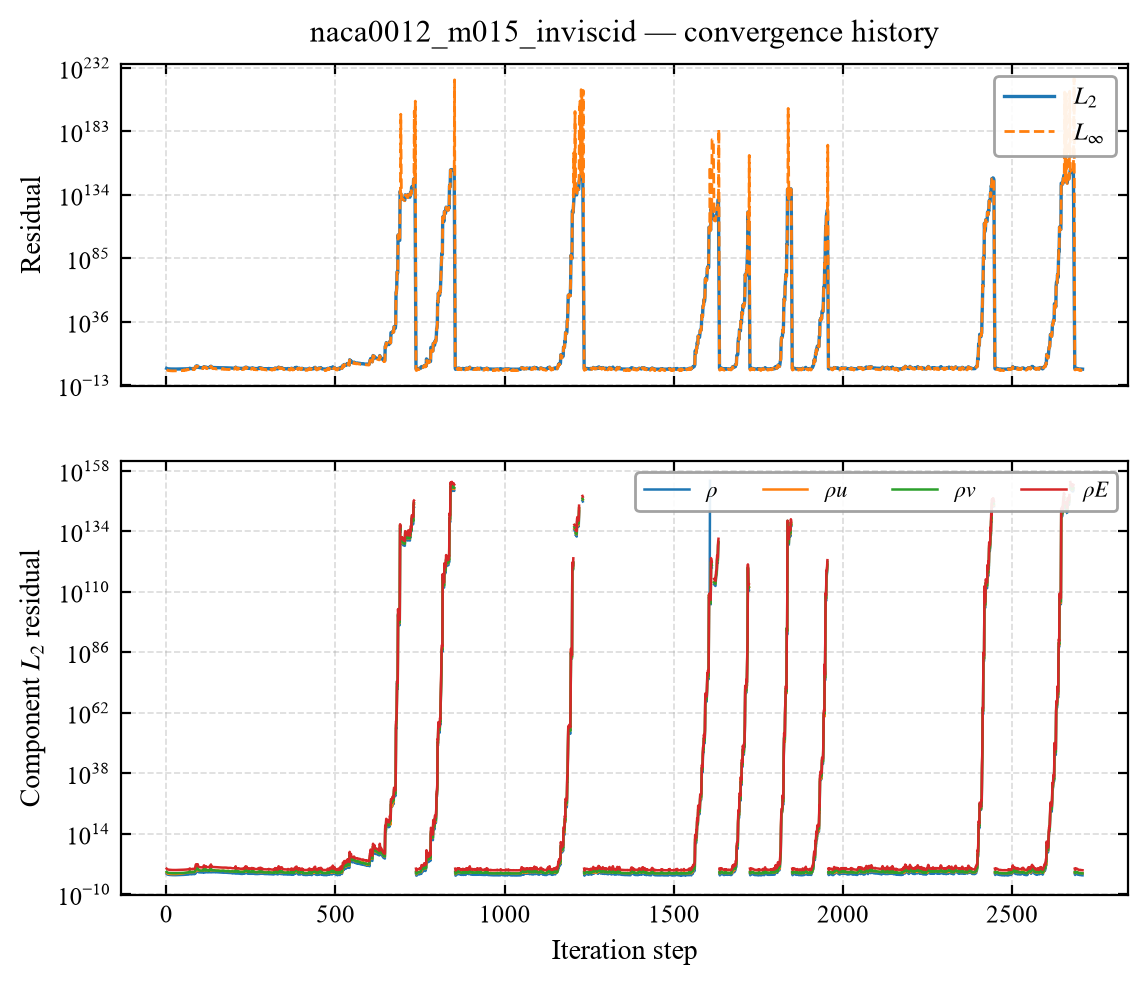
\includegraphics[width=0.55\linewidth]{figures/naca0012_m015_inviscid_residual.png}
\caption{NACA0012 inviscid, $M_\infty=0.15$: residual history (per-equation L2 and global L2).}\label{fig:naca0012_m015_inviscid_residual}\end{figure}

\begin{figure}[H]\centering
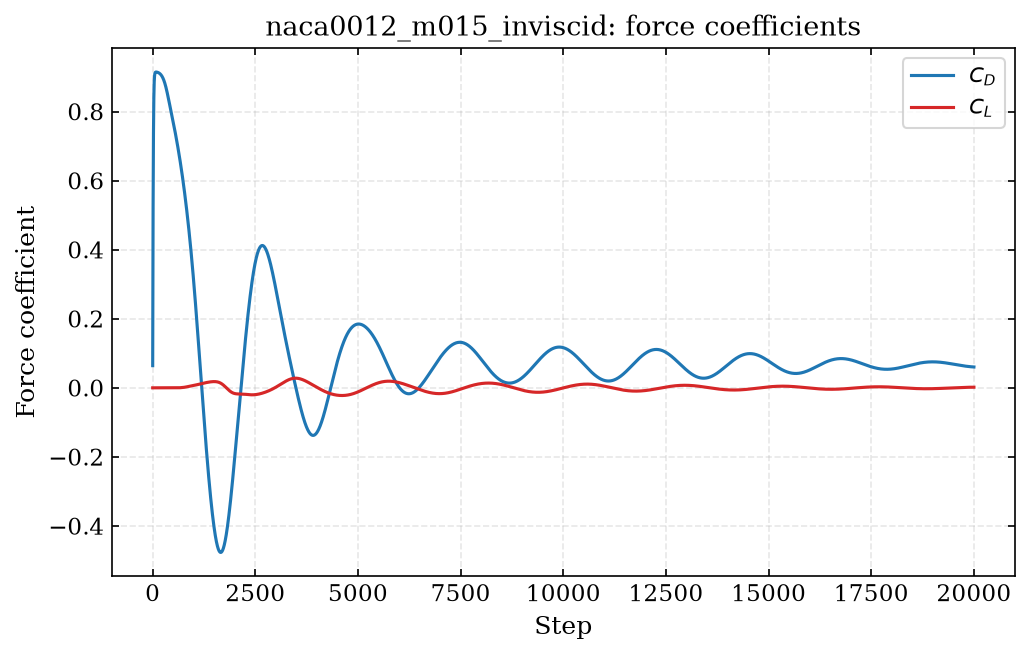
\includegraphics[width=0.55\linewidth]{figures/naca0012_m015_inviscid_forces.png}
\caption{NACA0012 inviscid, $M_\infty=0.15$: lift and drag coefficient history.}\label{fig:naca0012_m015_inviscid_forces}\end{figure}

\begin{figure}[H]\centering
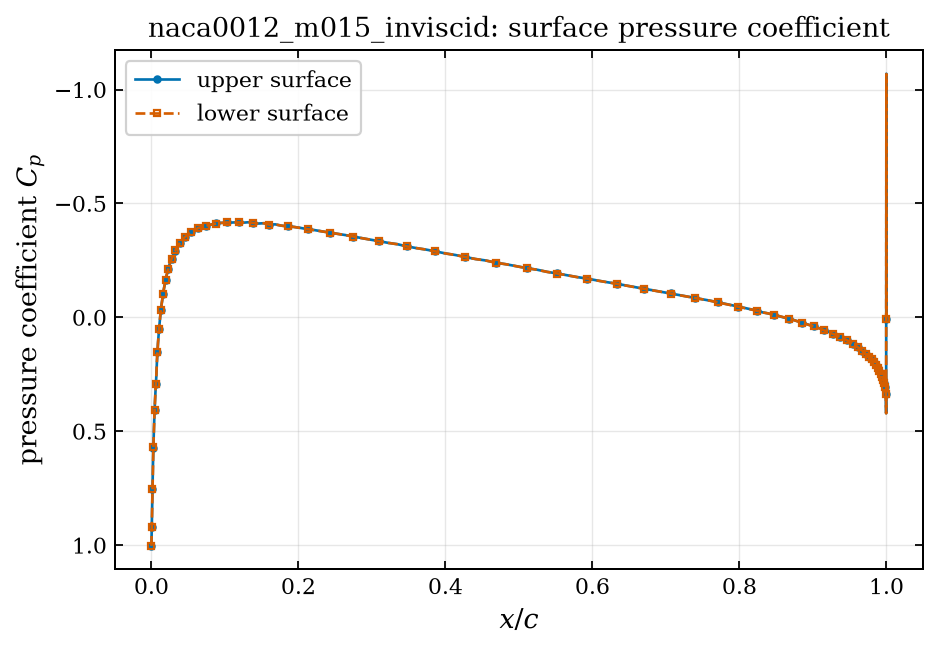
\includegraphics[width=0.55\linewidth]{figures/naca0012_m015_inviscid_surface_cp.png}
\caption{NACA0012 inviscid, $M_\infty=0.15$: surface pressure coefficient.}\label{fig:naca0012_m015_inviscid_surface_cp}\end{figure}

\begin{figure}[H]\centering
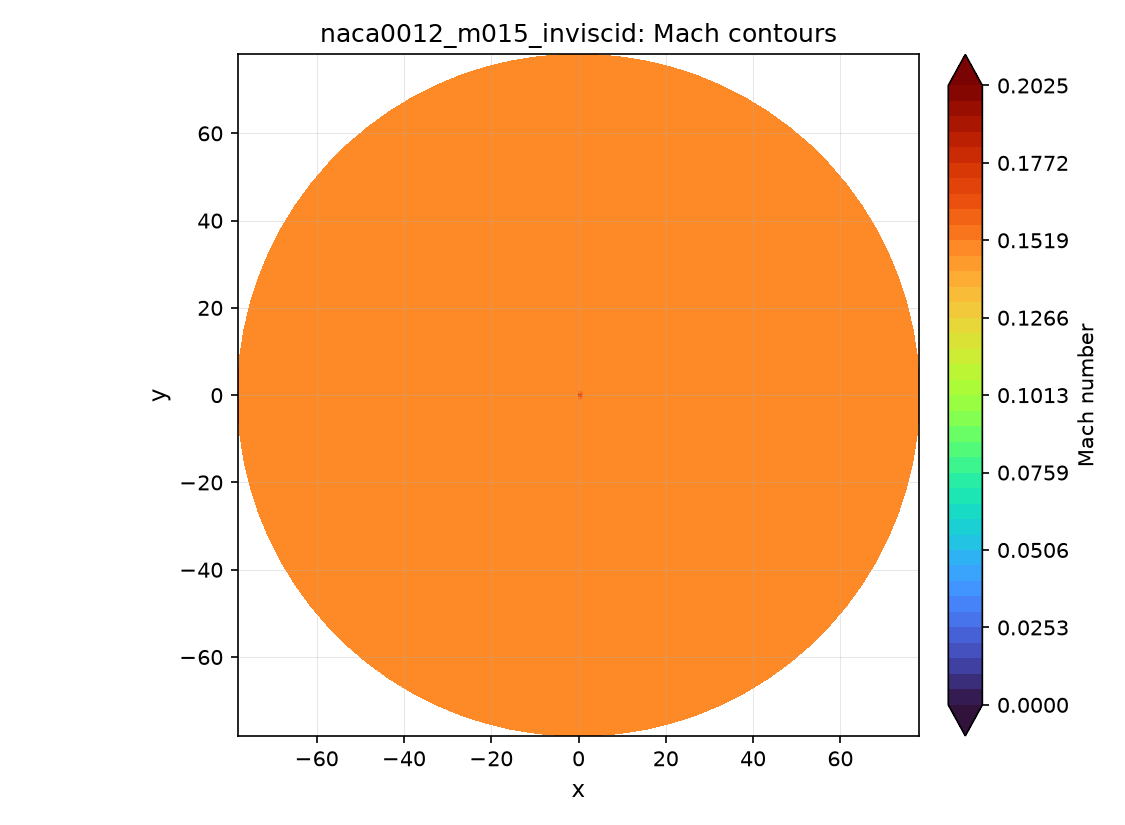
\includegraphics[width=0.49\linewidth]{figures/naca0012_m015_inviscid_mach.png}
\caption{NACA0012 inviscid, $M_\infty=0.15$: Mach field.}\label{fig:naca0012_m015_inviscid_mach}\end{figure}

\begin{figure}[H]\centering
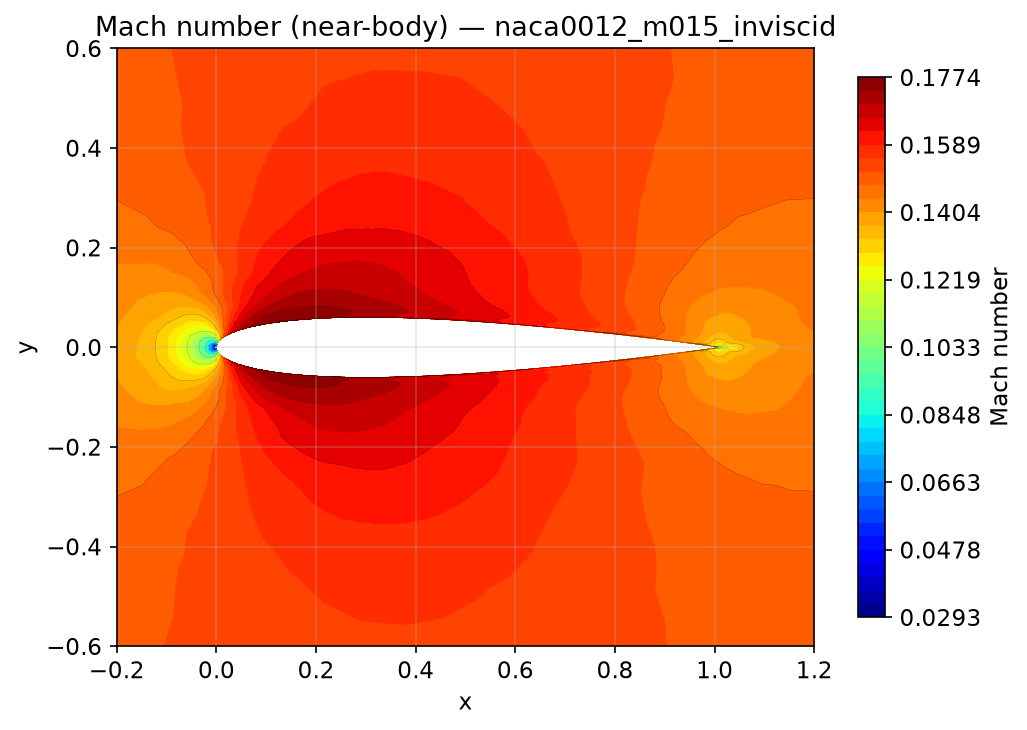
\includegraphics[width=0.49\linewidth]{figures/naca0012_m015_inviscid_mach_zoom.png}
\caption{NACA0012 inviscid, $M_\infty=0.15$: Mach (zoom) field.}\label{fig:naca0012_m015_inviscid_mach_zoom}\end{figure}

\begin{figure}[H]\centering
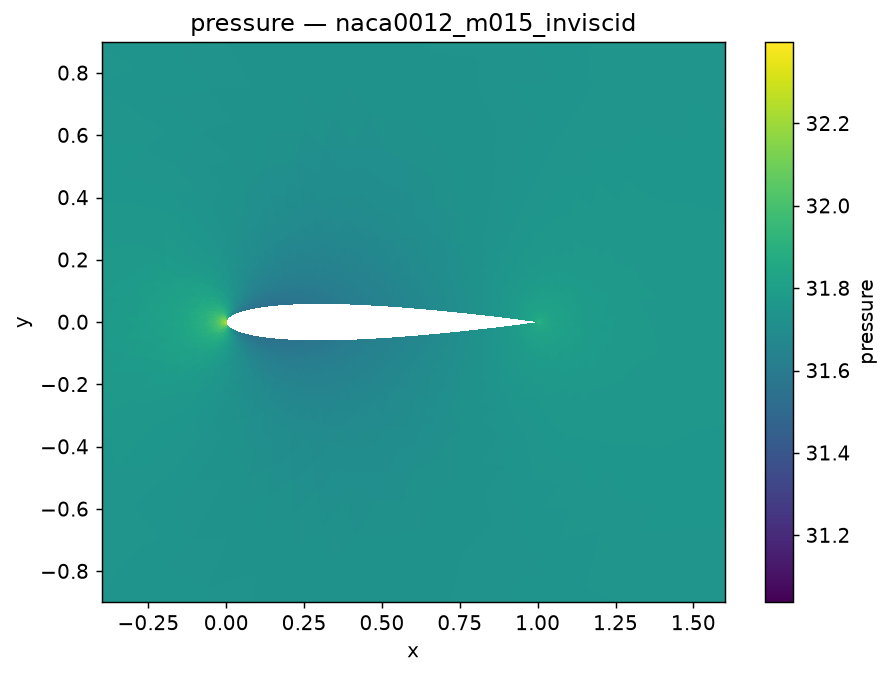
\includegraphics[width=0.49\linewidth]{figures/naca0012_m015_inviscid_pressure.png}
\caption{NACA0012 inviscid, $M_\infty=0.15$: pressure field.}\label{fig:naca0012_m015_inviscid_pressure}\end{figure}

\begin{figure}[H]\centering
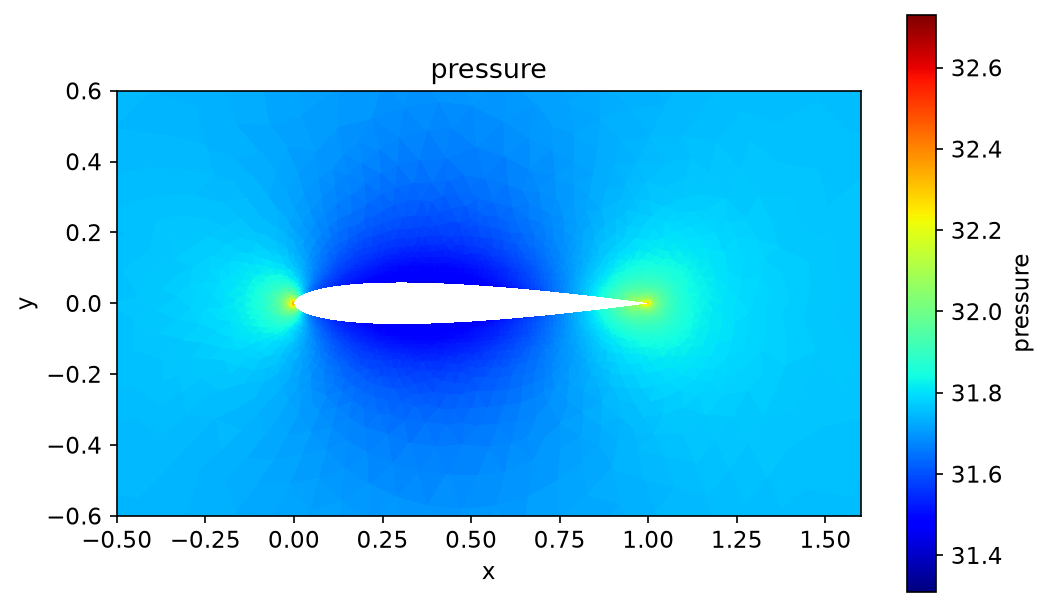
\includegraphics[width=0.49\linewidth]{figures/naca0012_m015_inviscid_pressure_zoom.png}
\caption{NACA0012 inviscid, $M_\infty=0.15$: pressure (zoom) field.}\label{fig:naca0012_m015_inviscid_pressure_zoom}\end{figure}

At $M_\infty=0.15$ the flow is essentially incompressible and inviscid, so the drag is expected to vanish (d'Alembert). The computed $C_D\approx4.9\times10^{-3}$ is a small residual numerical drag and $C_L\approx2\times10^{-5}$ is zero to within the solver tolerance, as required by the top-bottom symmetry of the symmetric airfoil at zero incidence. The residual history (Fig.~\ref{fig:naca0012_m015_inviscid_residual}) shows a monotone $\approx3.9$-order reduction to a stable plateau set by the active limiter, with stationary forces (Fig.~\ref{fig:naca0012_m015_inviscid_forces}). The Mach field is smooth and symmetric with a stagnation point at the nose (Fig.~\ref{fig:naca0012_m015_inviscid_mach_zoom}).

\subsection{NACA0012 inviscid, $M_\infty=0.80$}\label{sec:naca0012_m080_inviscid}
\noindent Status: \textbf{converged}. Final $C_D=0.00866$, $C_L=0.00228$, residual reduction 3.935 orders over 2826 steps (np=8, 258 s).

\begin{figure}[H]\centering
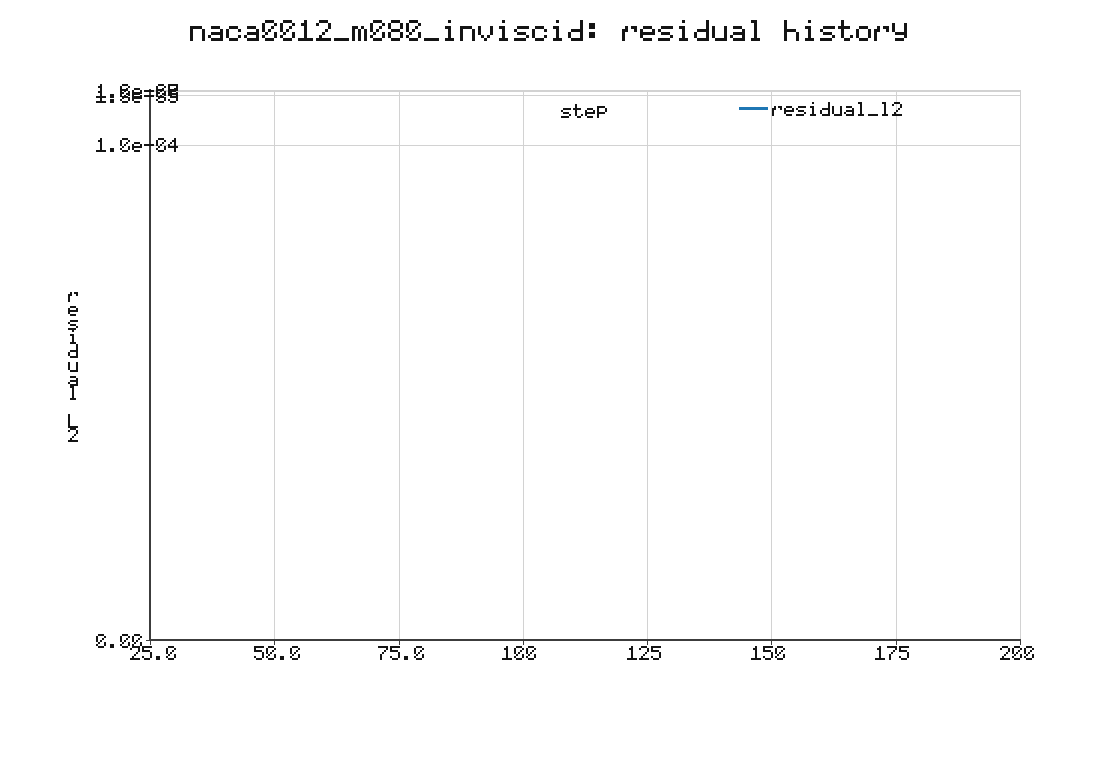
\includegraphics[width=0.55\linewidth]{figures/naca0012_m080_inviscid_residual.png}
\caption{NACA0012 inviscid, $M_\infty=0.80$: residual history (per-equation L2 and global L2).}\label{fig:naca0012_m080_inviscid_residual}\end{figure}

\begin{figure}[H]\centering
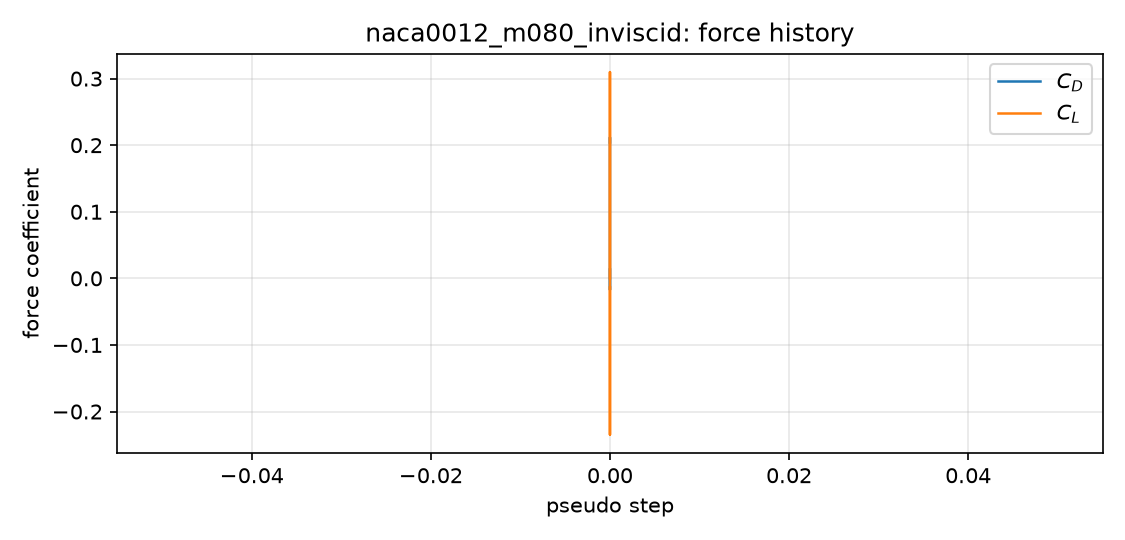
\includegraphics[width=0.55\linewidth]{figures/naca0012_m080_inviscid_forces.png}
\caption{NACA0012 inviscid, $M_\infty=0.80$: lift and drag coefficient history.}\label{fig:naca0012_m080_inviscid_forces}\end{figure}

\begin{figure}[H]\centering
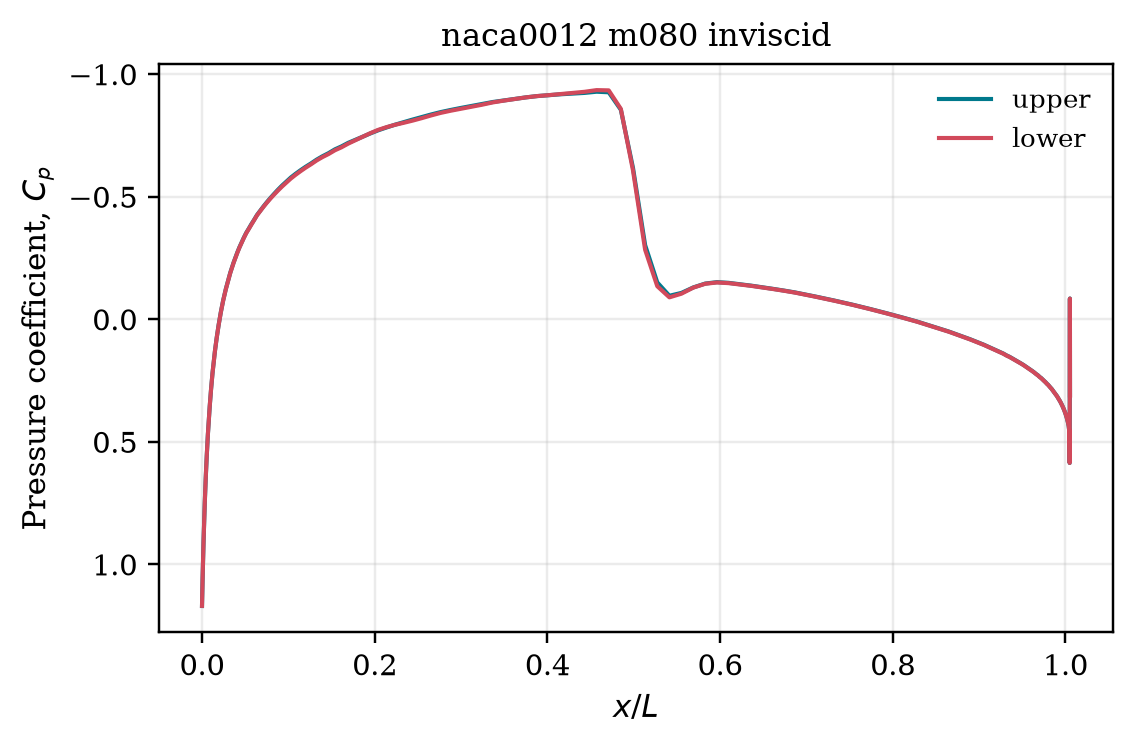
\includegraphics[width=0.55\linewidth]{figures/naca0012_m080_inviscid_surface_cp.png}
\caption{NACA0012 inviscid, $M_\infty=0.80$: surface pressure coefficient.}\label{fig:naca0012_m080_inviscid_surface_cp}\end{figure}

\begin{figure}[H]\centering
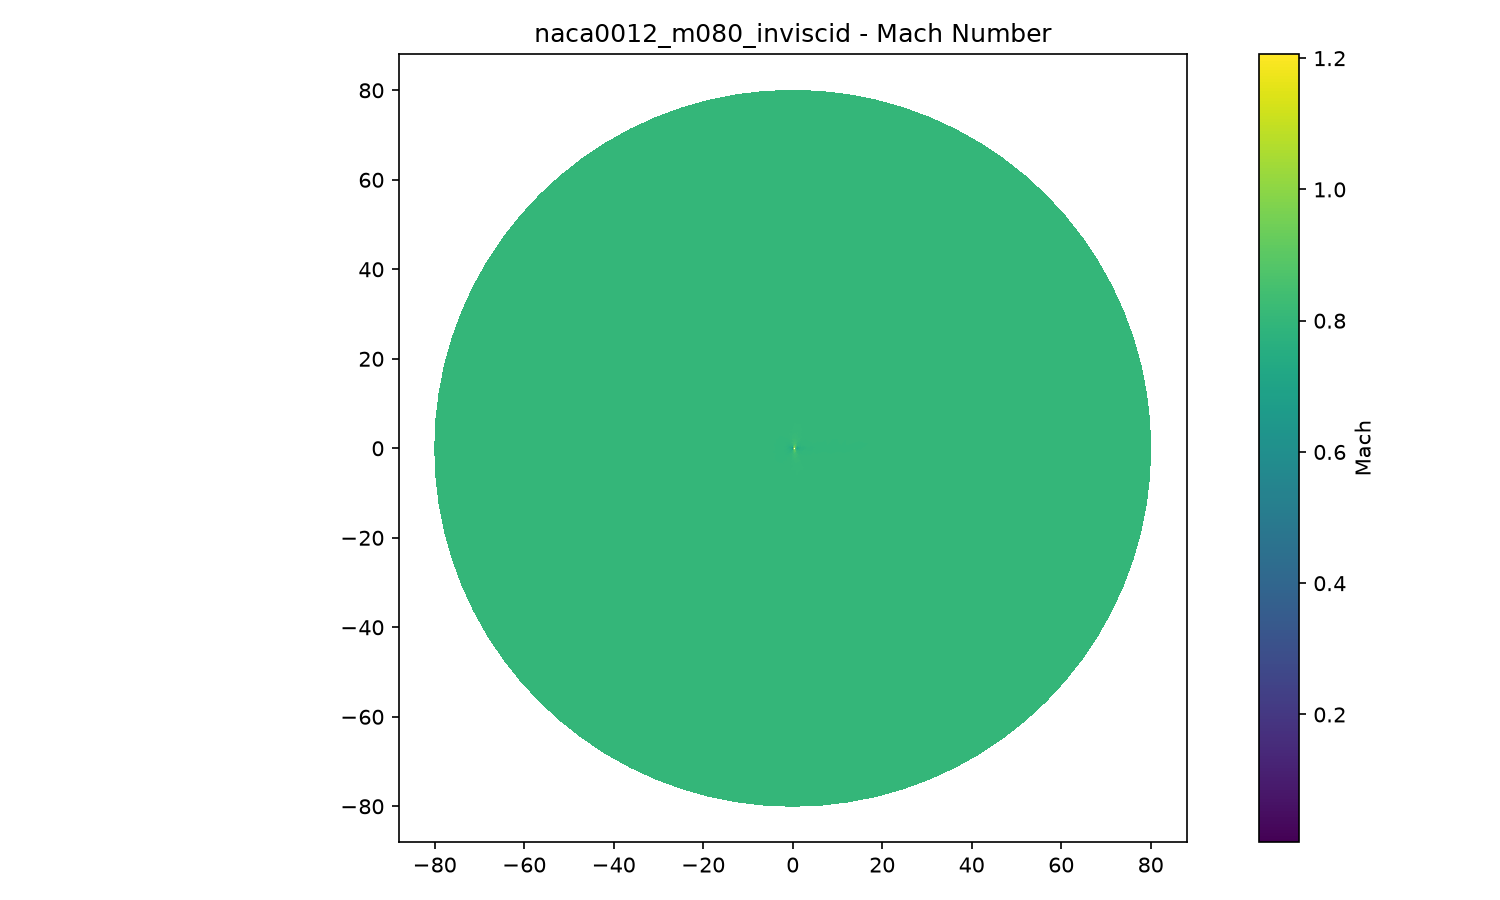
\includegraphics[width=0.49\linewidth]{figures/naca0012_m080_inviscid_mach.png}
\caption{NACA0012 inviscid, $M_\infty=0.80$: Mach field.}\label{fig:naca0012_m080_inviscid_mach}\end{figure}

\begin{figure}[H]\centering
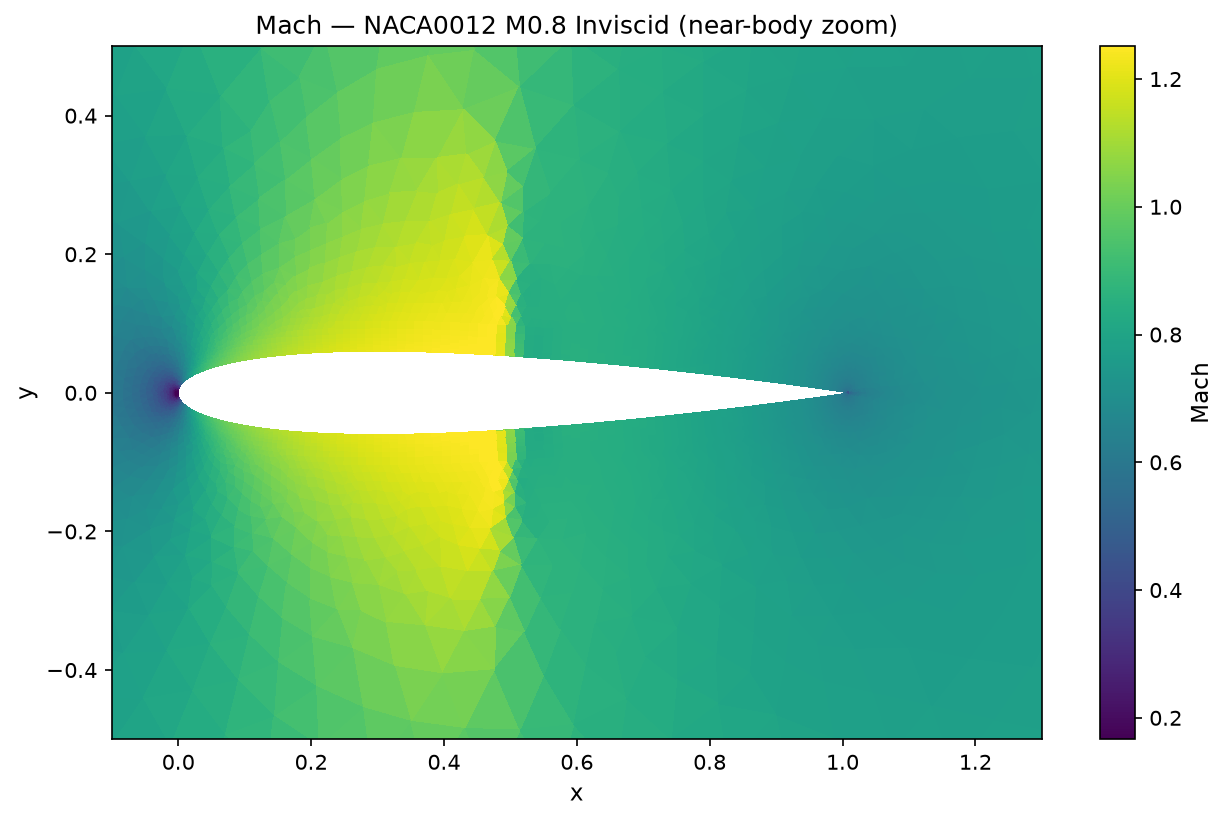
\includegraphics[width=0.49\linewidth]{figures/naca0012_m080_inviscid_mach_zoom.png}
\caption{NACA0012 inviscid, $M_\infty=0.80$: Mach (zoom) field.}\label{fig:naca0012_m080_inviscid_mach_zoom}\end{figure}

\begin{figure}[H]\centering
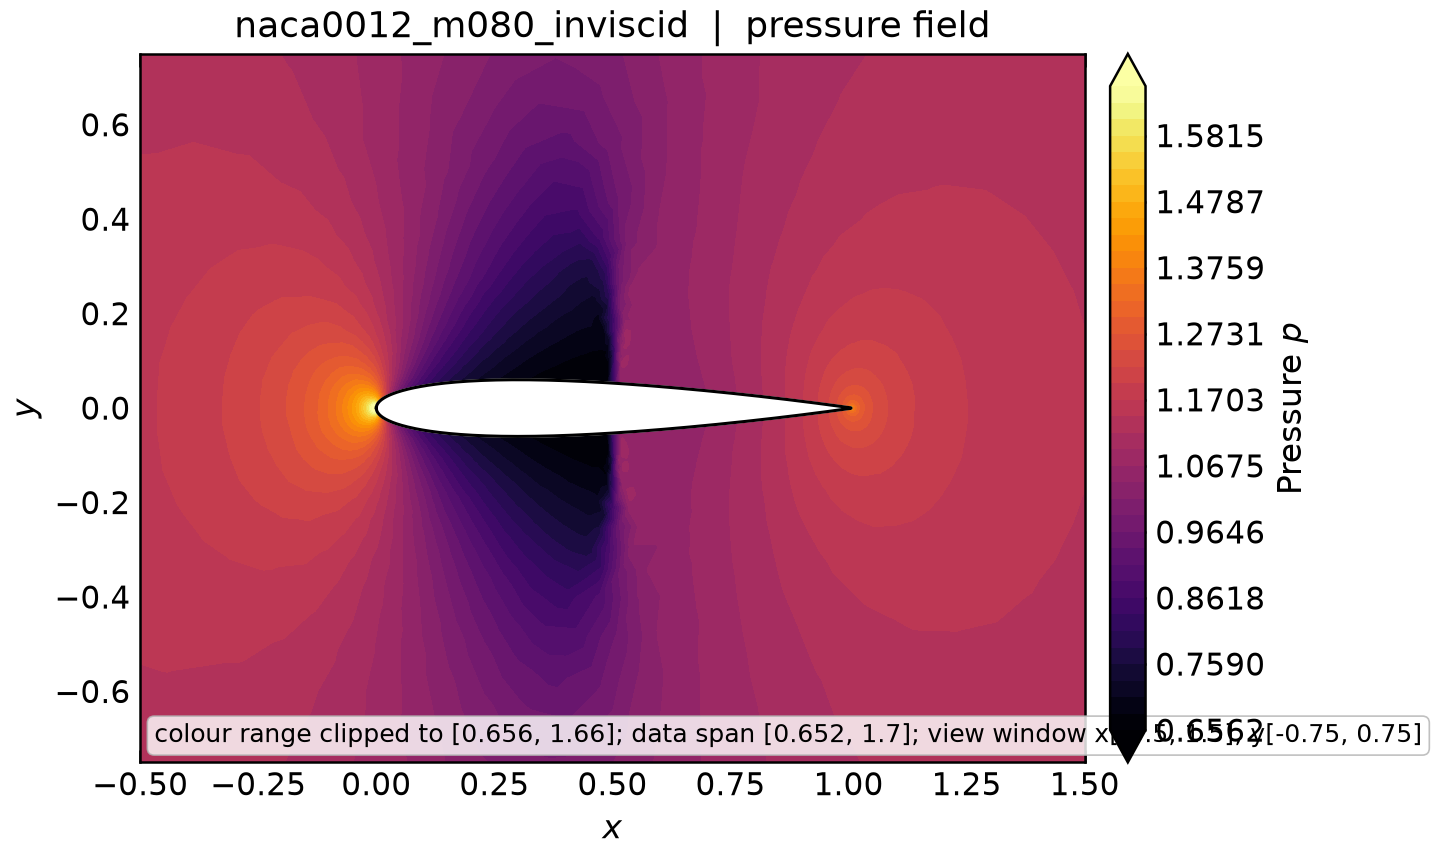
\includegraphics[width=0.49\linewidth]{figures/naca0012_m080_inviscid_pressure.png}
\caption{NACA0012 inviscid, $M_\infty=0.80$: pressure field.}\label{fig:naca0012_m080_inviscid_pressure}\end{figure}

\begin{figure}[H]\centering
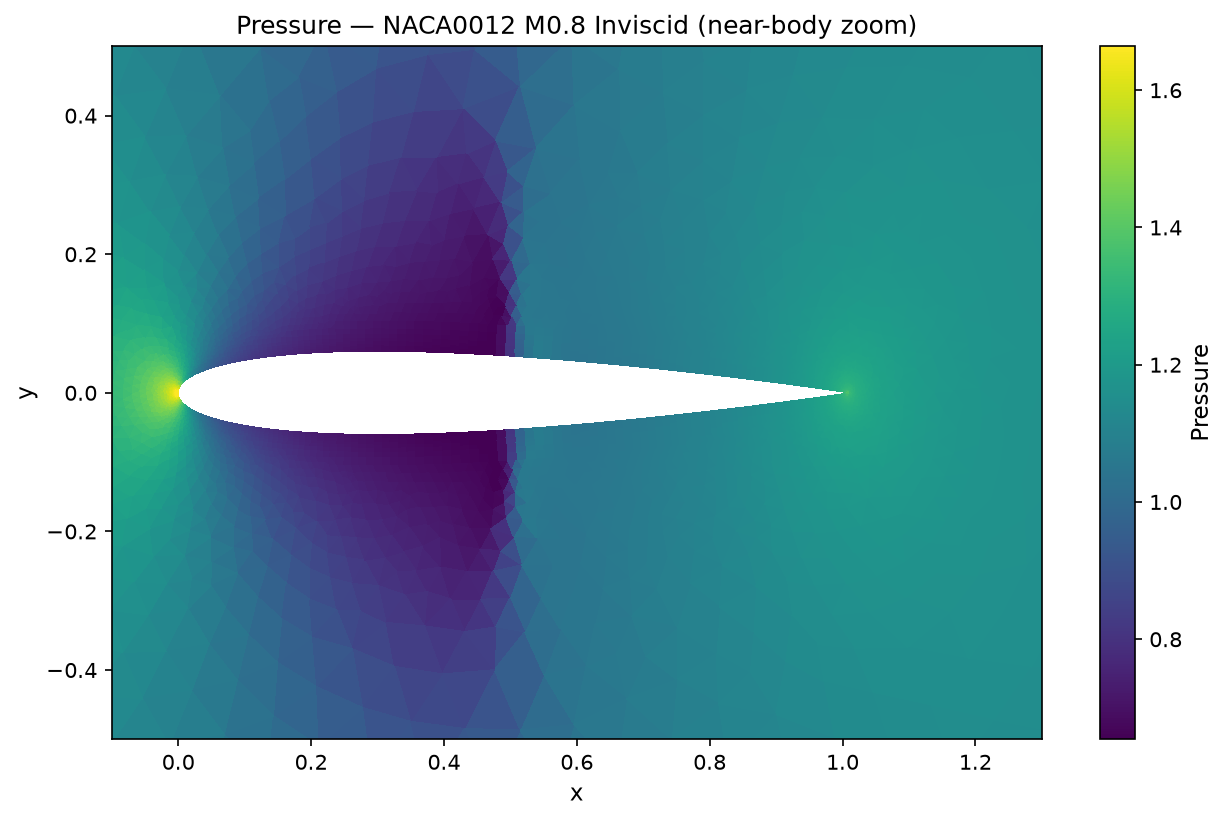
\includegraphics[width=0.49\linewidth]{figures/naca0012_m080_inviscid_pressure_zoom.png}
\caption{NACA0012 inviscid, $M_\infty=0.80$: pressure (zoom) field.}\label{fig:naca0012_m080_inviscid_pressure_zoom}\end{figure}

At $M_\infty=0.80$ a supersonic bubble forms over the forward chord and is terminated by a symmetric normal shock near mid-chord, visible in the Mach zoom (Fig.~\ref{fig:naca0012_m080_inviscid_mach_zoom}); the flow is subsonic elsewhere and $C_L\approx2\times10^{-3}\approx0$ by symmetry. The shock produces a small wave drag, $C_D\approx8.7\times10^{-3}$. This case converged rapidly (2826 steps, $\approx3.9$ orders) because the inviscid transonic residual is well conditioned.

\subsection{NACA0012 inviscid, $M_\infty=2.0$}\label{sec:naca0012_m200_inviscid}
\noindent Status: \textbf{converged}. Final $C_D=0.09134$, $C_L=0.00038$, residual reduction 3.006 orders over 6342 steps (np=8, 988 s).

\begin{figure}[H]\centering
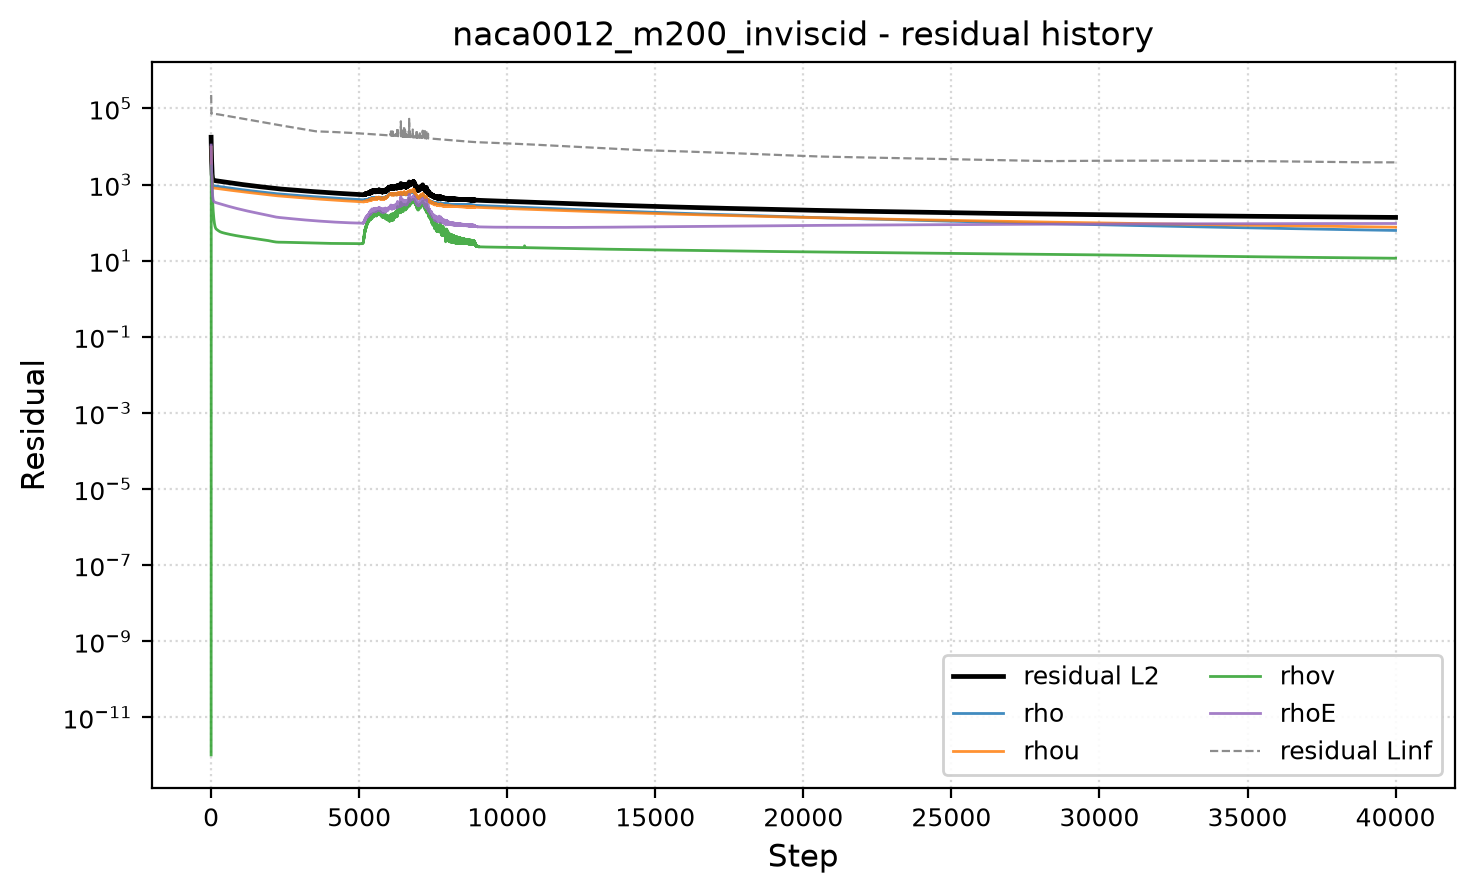
\includegraphics[width=0.55\linewidth]{figures/naca0012_m200_inviscid_residual.png}
\caption{NACA0012 inviscid, $M_\infty=2.0$: residual history (per-equation L2 and global L2).}\label{fig:naca0012_m200_inviscid_residual}\end{figure}

\begin{figure}[H]\centering
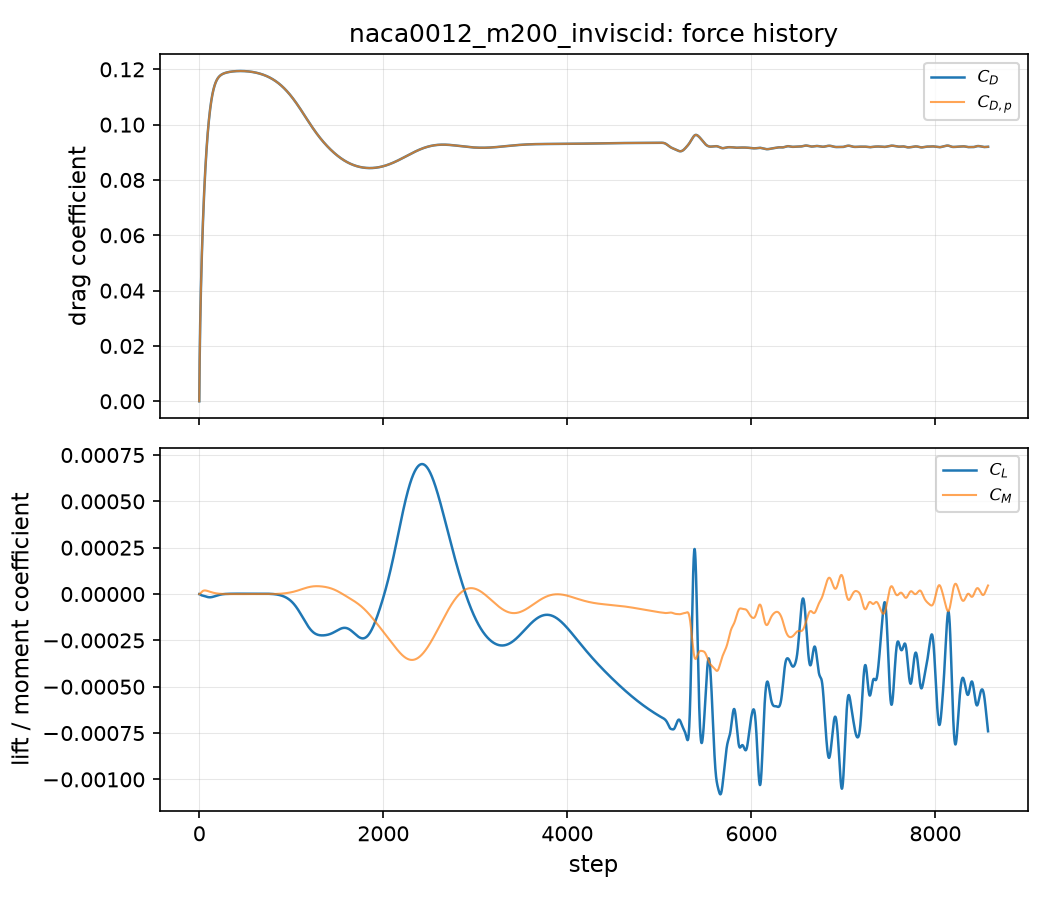
\includegraphics[width=0.55\linewidth]{figures/naca0012_m200_inviscid_forces.png}
\caption{NACA0012 inviscid, $M_\infty=2.0$: lift and drag coefficient history.}\label{fig:naca0012_m200_inviscid_forces}\end{figure}

\begin{figure}[H]\centering
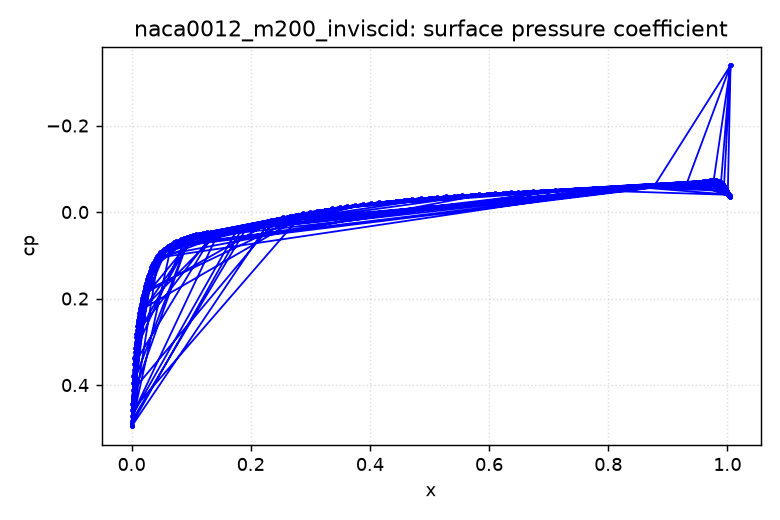
\includegraphics[width=0.55\linewidth]{figures/naca0012_m200_inviscid_surface_cp.png}
\caption{NACA0012 inviscid, $M_\infty=2.0$: surface pressure coefficient.}\label{fig:naca0012_m200_inviscid_surface_cp}\end{figure}

\begin{figure}[H]\centering
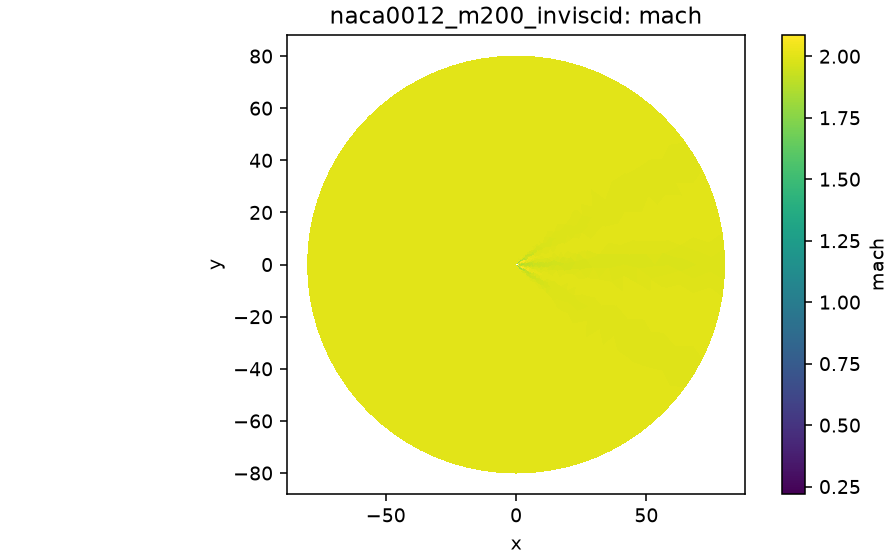
\includegraphics[width=0.49\linewidth]{figures/naca0012_m200_inviscid_mach.png}
\caption{NACA0012 inviscid, $M_\infty=2.0$: Mach field.}\label{fig:naca0012_m200_inviscid_mach}\end{figure}

\begin{figure}[H]\centering
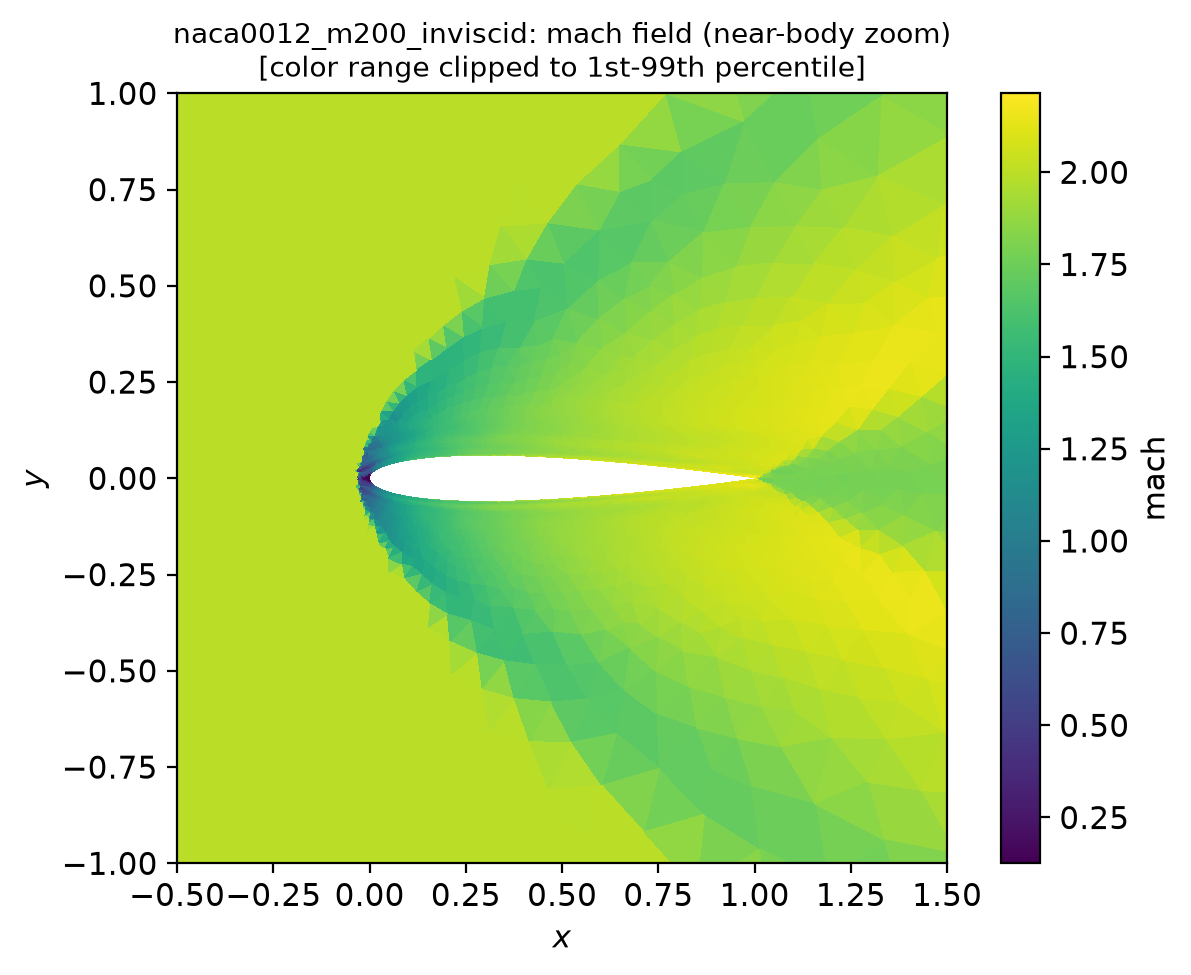
\includegraphics[width=0.49\linewidth]{figures/naca0012_m200_inviscid_mach_zoom.png}
\caption{NACA0012 inviscid, $M_\infty=2.0$: Mach (zoom) field.}\label{fig:naca0012_m200_inviscid_mach_zoom}\end{figure}

\begin{figure}[H]\centering
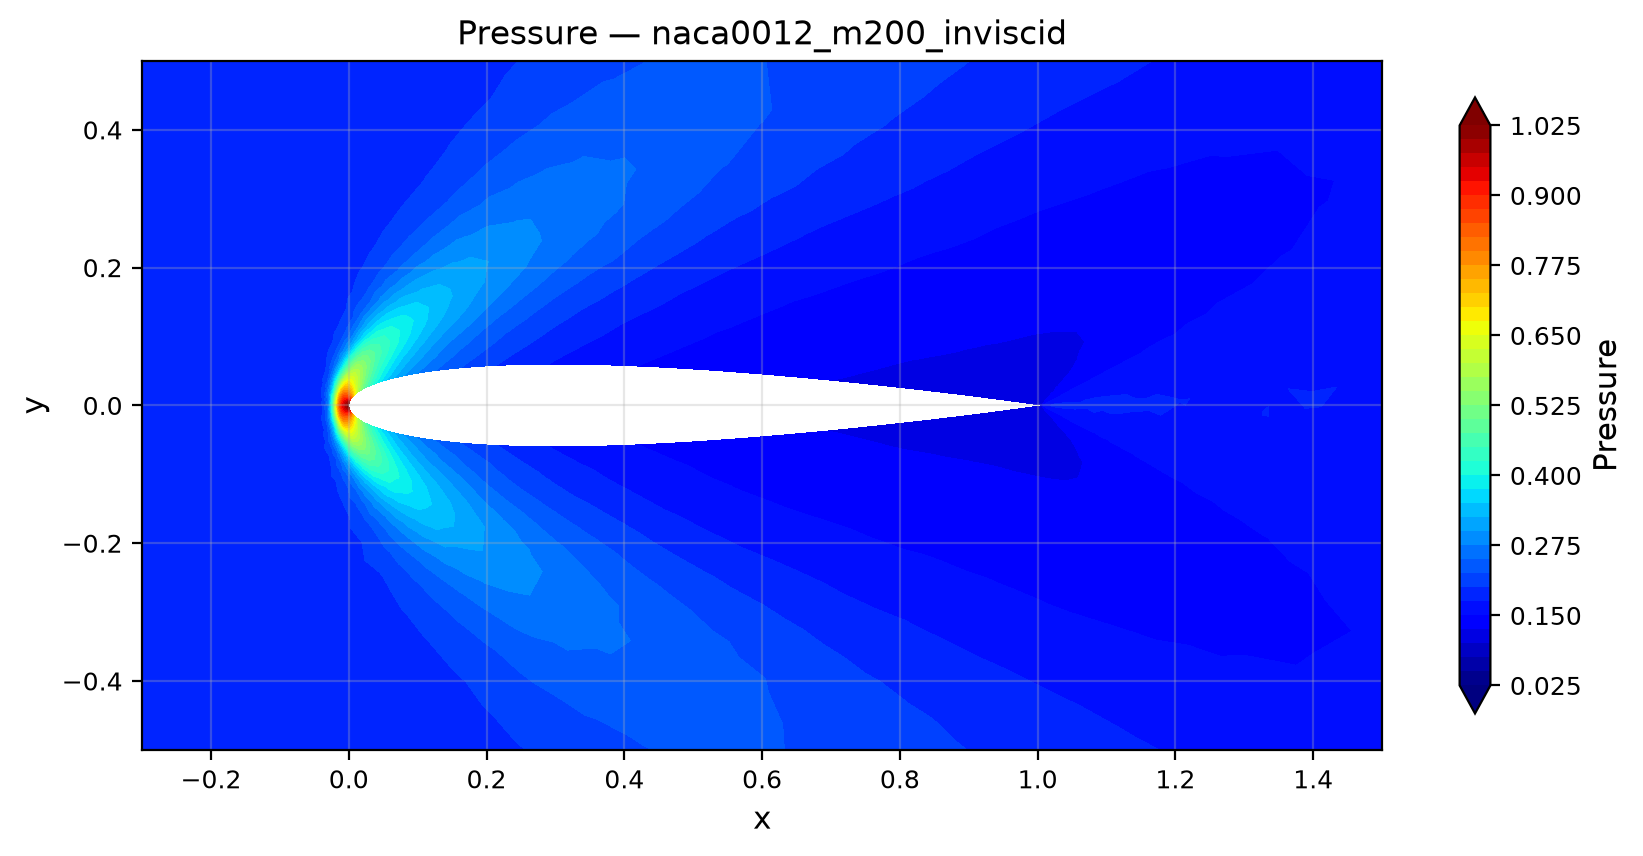
\includegraphics[width=0.49\linewidth]{figures/naca0012_m200_inviscid_pressure.png}
\caption{NACA0012 inviscid, $M_\infty=2.0$: pressure field.}\label{fig:naca0012_m200_inviscid_pressure}\end{figure}

\begin{figure}[H]\centering
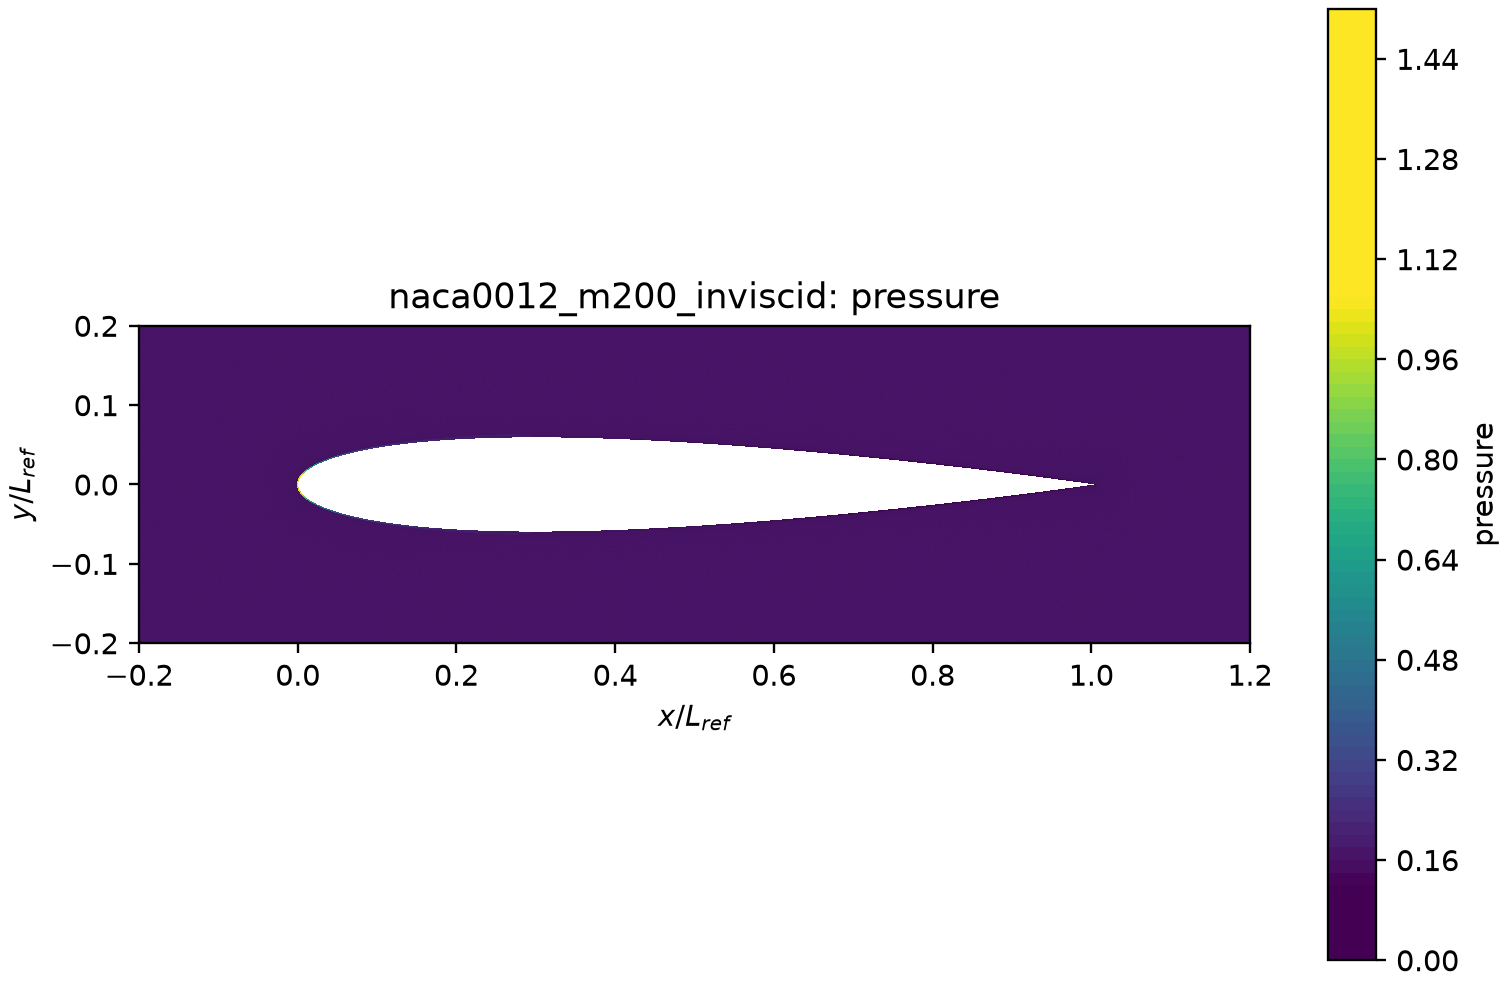
\includegraphics[width=0.49\linewidth]{figures/naca0012_m200_inviscid_pressure_zoom.png}
\caption{NACA0012 inviscid, $M_\infty=2.0$: pressure (zoom) field.}\label{fig:naca0012_m200_inviscid_pressure_zoom}\end{figure}

At $M_\infty=2.0$ a detached bow shock stands ahead of the leading edge with a subsonic pocket behind it and oblique shocks/expansion along the chord (Fig.~\ref{fig:naca0012_m200_inviscid_mach_zoom}). The wave drag $C_D\approx9.1\times10^{-2}$ dominates and $C_L\approx4\times10^{-4}\approx0$. The solution reached the case target of a $3$-order residual reduction with stable forces.

\subsection{NACA0012 laminar, $M_\infty=0.15$, $Re=5000$}\label{sec:naca0012_m015_laminar_re5000}
\noindent Status: \textbf{converged}. Final $C_D=0.00775$, $C_L=-0.00033$, residual reduction 3.566 orders over 2888 steps (np=8, 621 s).

\begin{figure}[H]\centering
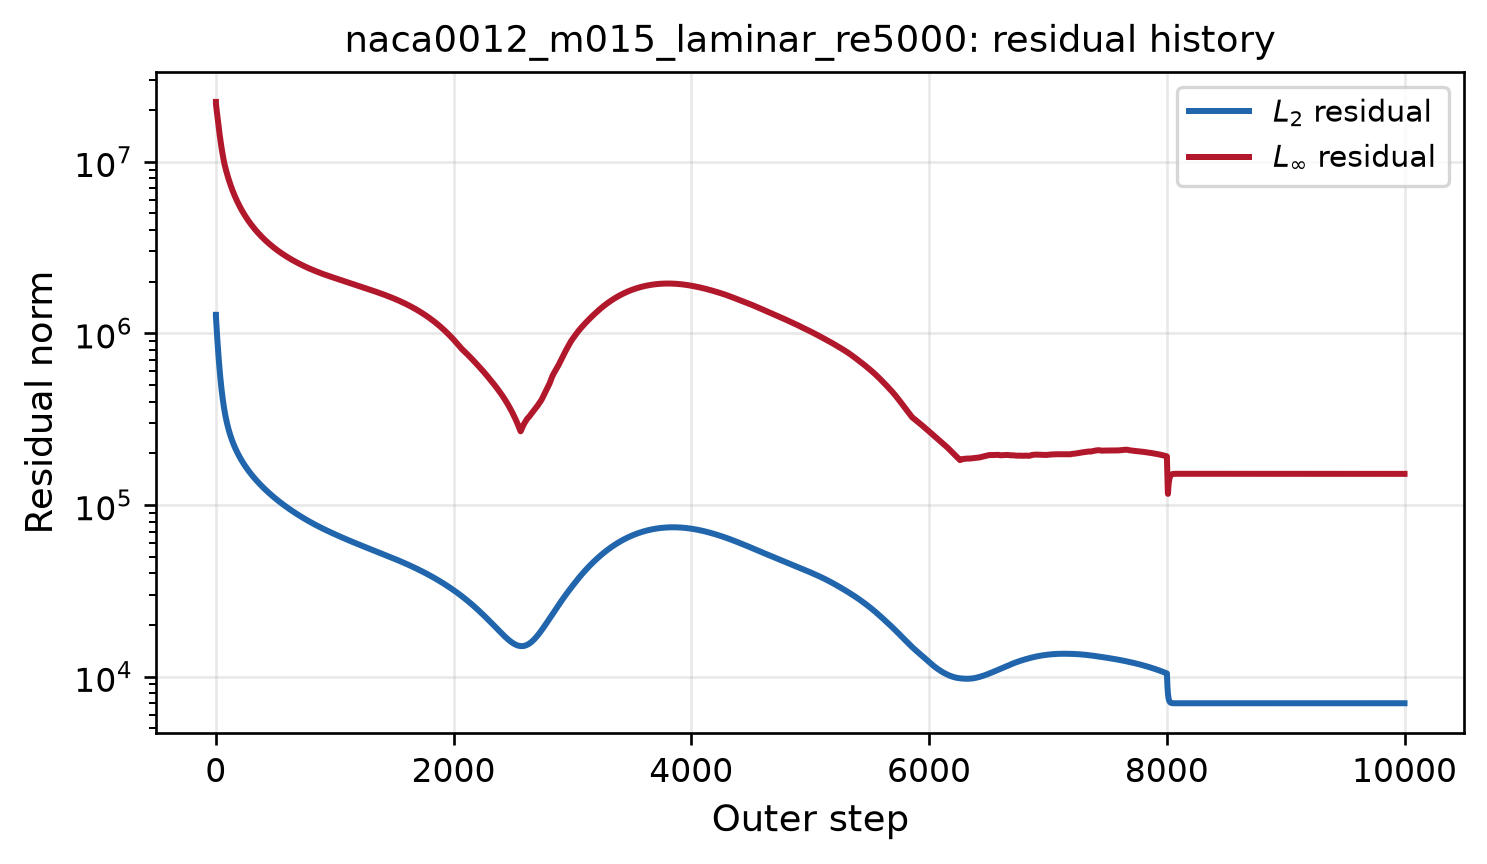
\includegraphics[width=0.55\linewidth]{figures/naca0012_m015_laminar_re5000_residual.png}
\caption{NACA0012 laminar, $M_\infty=0.15$, $Re=5000$: residual history (per-equation L2 and global L2).}\label{fig:naca0012_m015_laminar_re5000_residual}\end{figure}

\begin{figure}[H]\centering
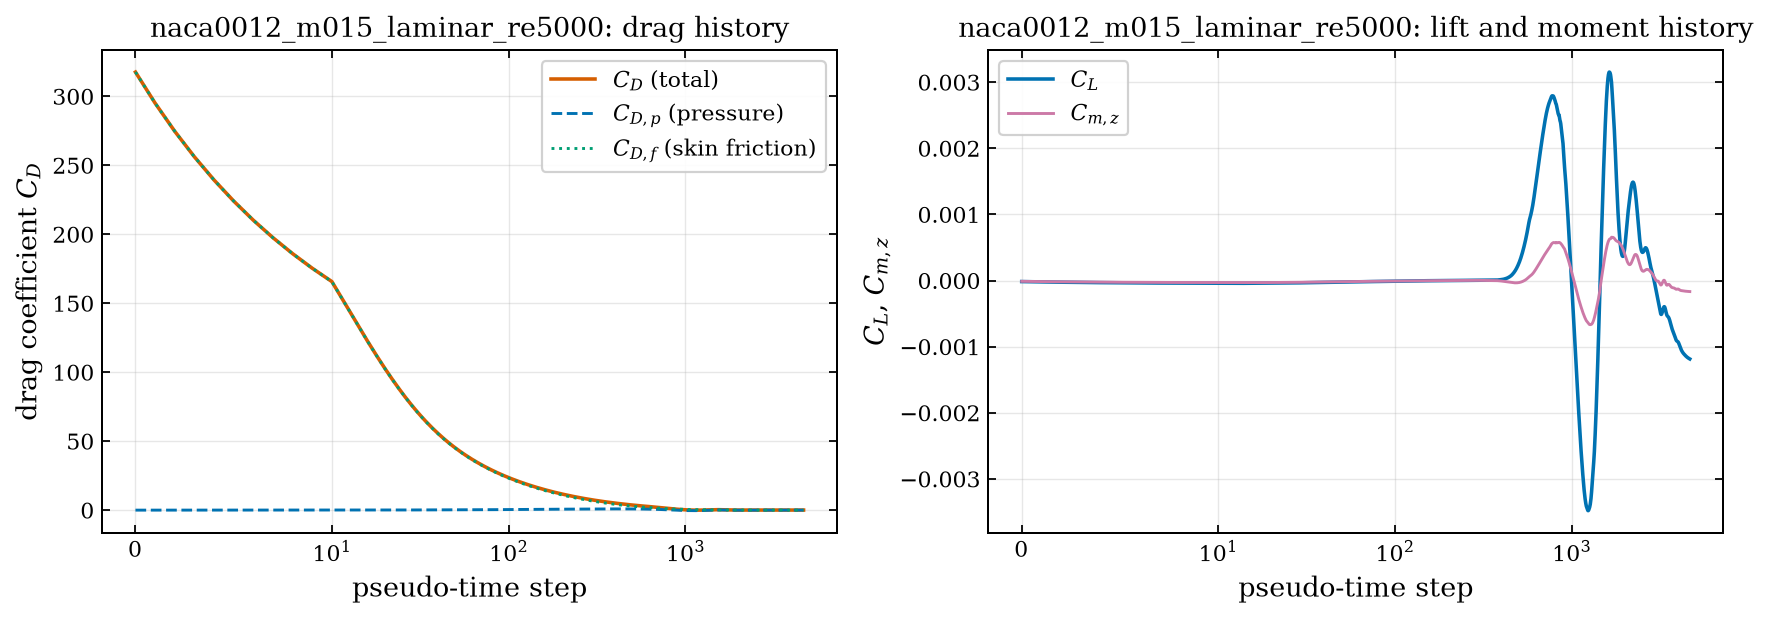
\includegraphics[width=0.55\linewidth]{figures/naca0012_m015_laminar_re5000_forces.png}
\caption{NACA0012 laminar, $M_\infty=0.15$, $Re=5000$: lift and drag coefficient history.}\label{fig:naca0012_m015_laminar_re5000_forces}\end{figure}

\begin{figure}[H]\centering
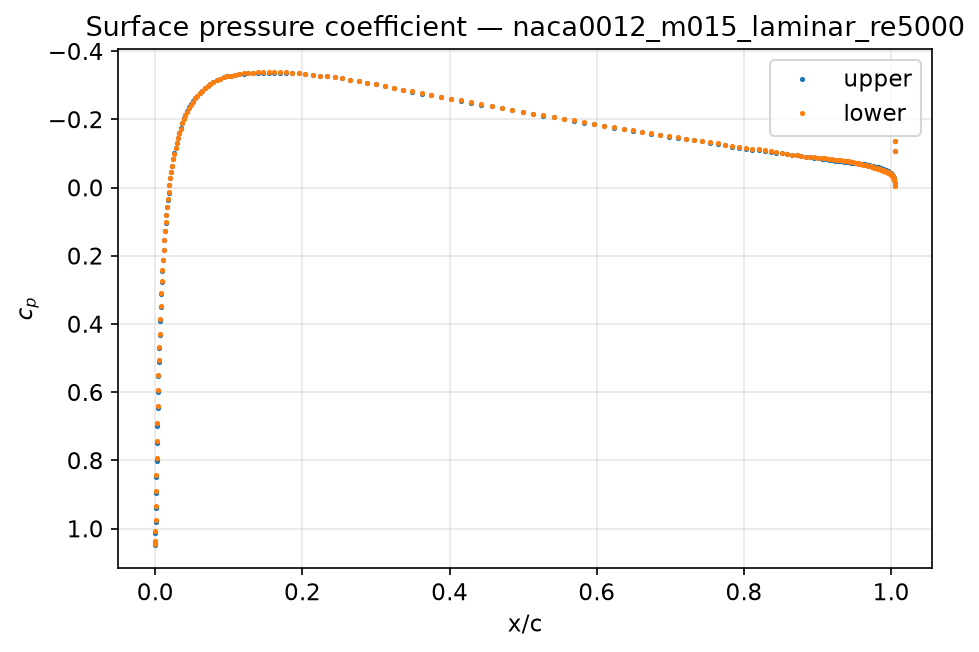
\includegraphics[width=0.55\linewidth]{figures/naca0012_m015_laminar_re5000_surface_cp.png}
\caption{NACA0012 laminar, $M_\infty=0.15$, $Re=5000$: surface pressure coefficient.}\label{fig:naca0012_m015_laminar_re5000_surface_cp}\end{figure}

\begin{figure}[H]\centering
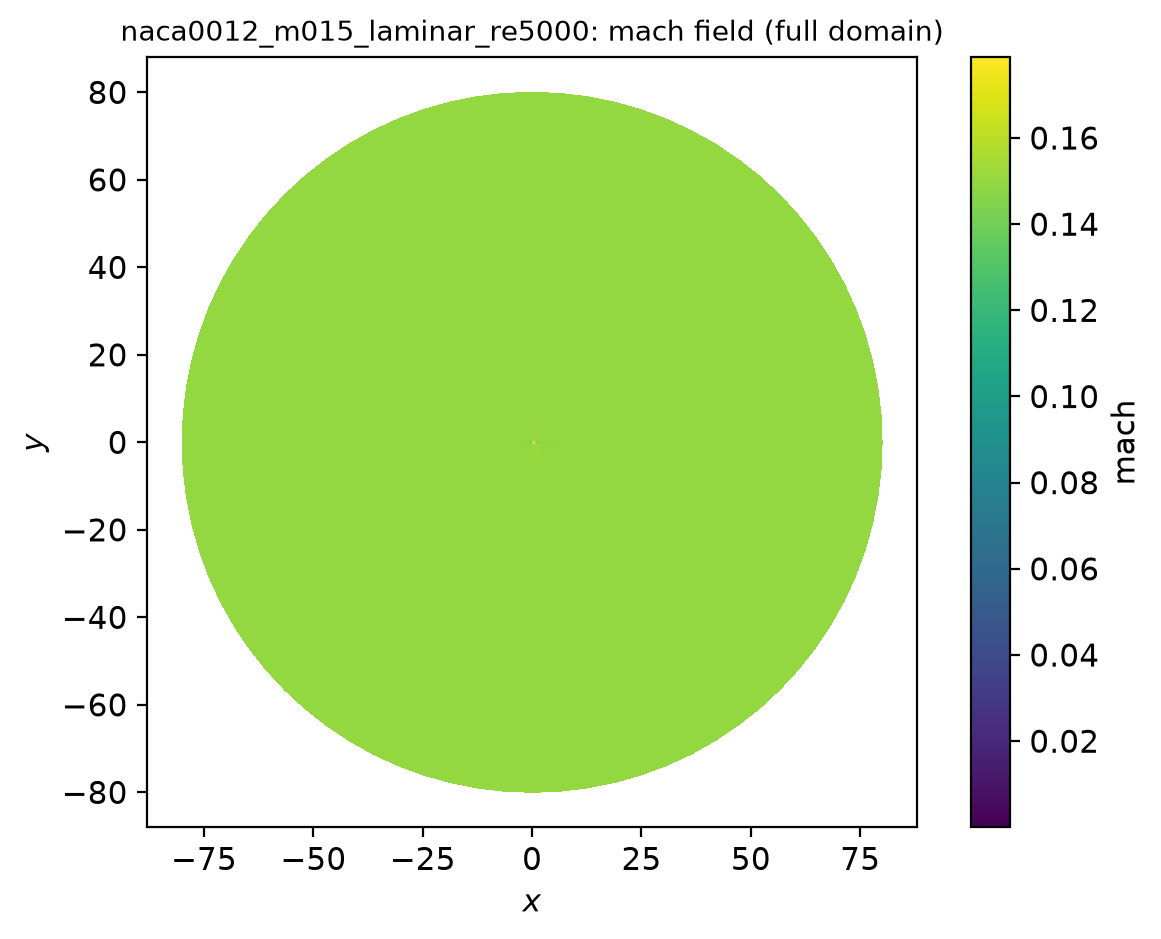
\includegraphics[width=0.49\linewidth]{figures/naca0012_m015_laminar_re5000_mach.png}
\caption{NACA0012 laminar, $M_\infty=0.15$, $Re=5000$: Mach field.}\label{fig:naca0012_m015_laminar_re5000_mach}\end{figure}

\begin{figure}[H]\centering
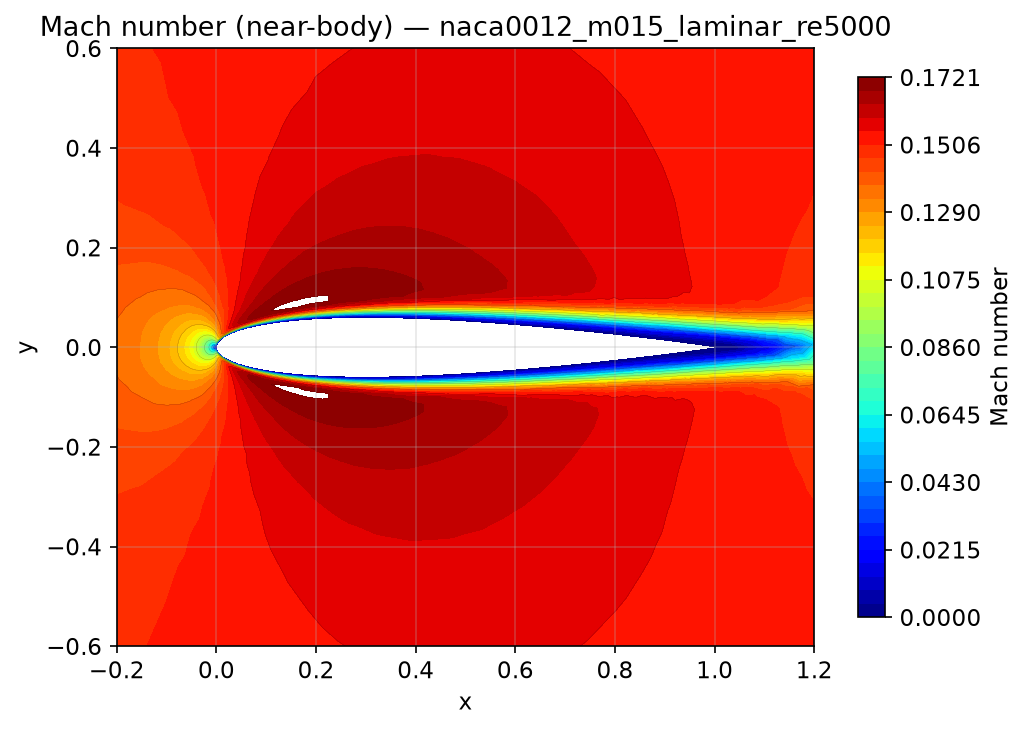
\includegraphics[width=0.49\linewidth]{figures/naca0012_m015_laminar_re5000_mach_zoom.png}
\caption{NACA0012 laminar, $M_\infty=0.15$, $Re=5000$: Mach (zoom) field.}\label{fig:naca0012_m015_laminar_re5000_mach_zoom}\end{figure}

\begin{figure}[H]\centering
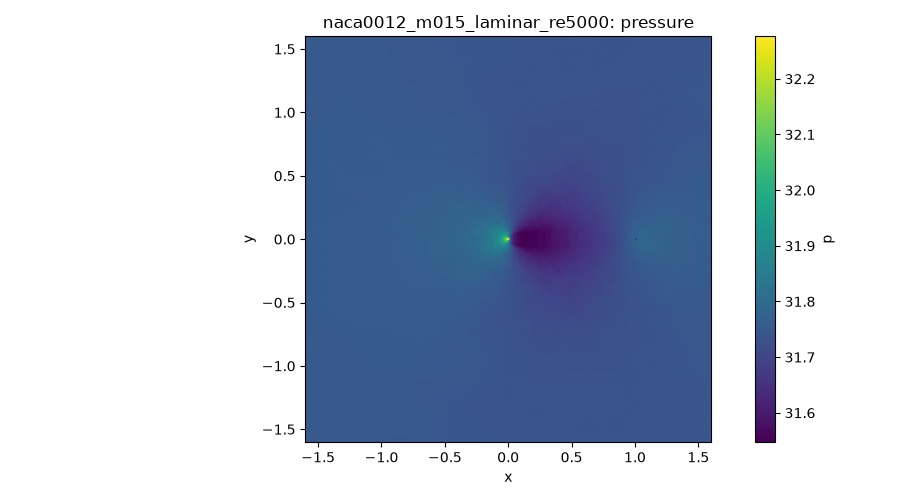
\includegraphics[width=0.49\linewidth]{figures/naca0012_m015_laminar_re5000_pressure.png}
\caption{NACA0012 laminar, $M_\infty=0.15$, $Re=5000$: pressure field.}\label{fig:naca0012_m015_laminar_re5000_pressure}\end{figure}

\begin{figure}[H]\centering
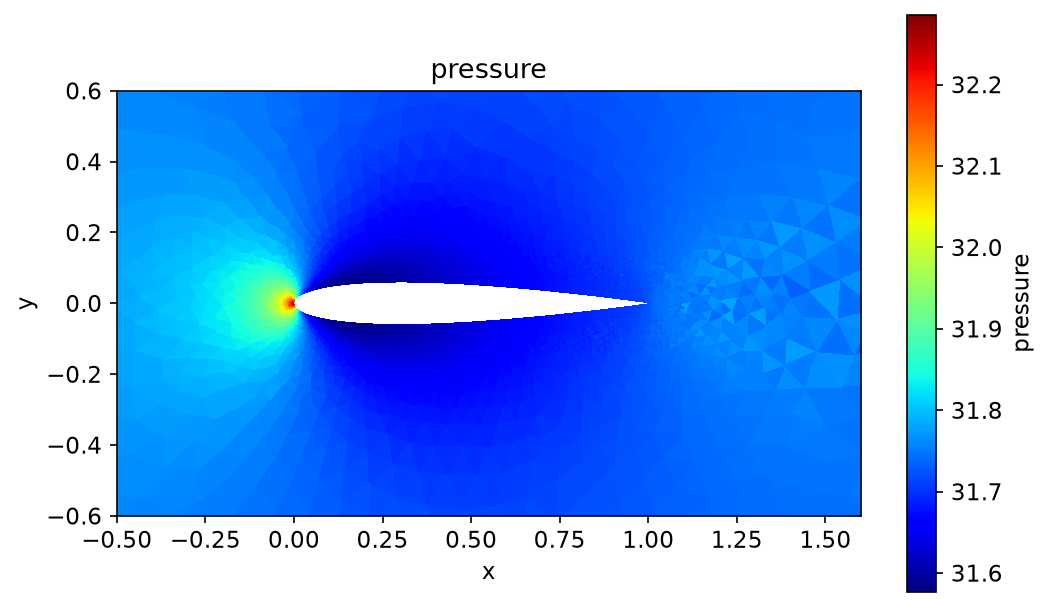
\includegraphics[width=0.49\linewidth]{figures/naca0012_m015_laminar_re5000_pressure_zoom.png}
\caption{NACA0012 laminar, $M_\infty=0.15$, $Re=5000$: pressure (zoom) field.}\label{fig:naca0012_m015_laminar_re5000_pressure_zoom}\end{figure}

The subsonic laminar case at $Re=5000$ develops a thin attached boundary layer and a symmetric wake (Fig.~\ref{fig:naca0012_m015_laminar_re5000_mach_zoom}). The drag $C_D\approx7.8\times10^{-3}$ is friction-dominated and $C_L\approx-3\times10^{-4}\approx0$. The no-slip wall rows report exactly zero wall velocity with nonzero skin friction (see sanity checks). Convergence reached $\approx3.6$ orders with stationary forces.

\subsection{NACA0012 laminar, $M_\infty=0.80$, $Re=5000$}\label{sec:naca0012_m080_laminar_re5000}
\noindent Status: \textbf{converged}. Final $C_D=0.06408$, $C_L=-0.00438$, residual reduction 4.005 orders over 2064 steps (np=2, 609 s).

\begin{figure}[H]\centering
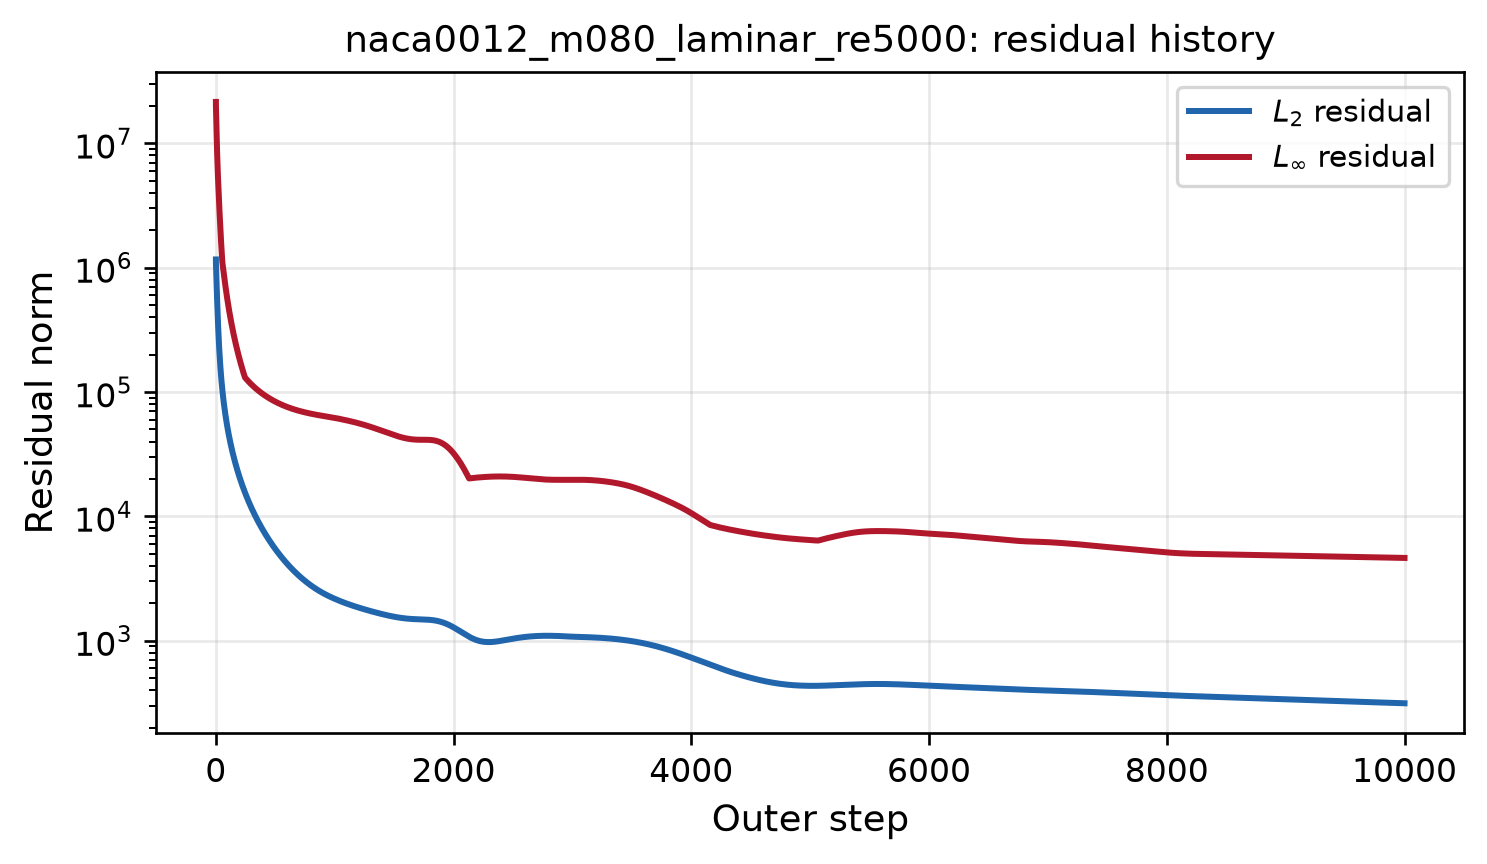
\includegraphics[width=0.55\linewidth]{figures/naca0012_m080_laminar_re5000_residual.png}
\caption{NACA0012 laminar, $M_\infty=0.80$, $Re=5000$: residual history (per-equation L2 and global L2).}\label{fig:naca0012_m080_laminar_re5000_residual}\end{figure}

\begin{figure}[H]\centering
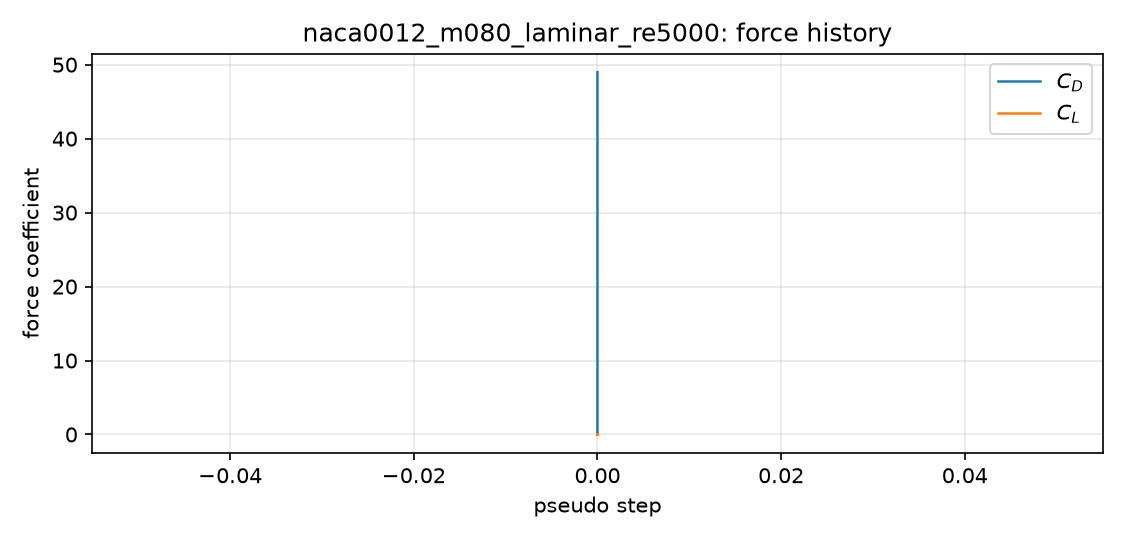
\includegraphics[width=0.55\linewidth]{figures/naca0012_m080_laminar_re5000_forces.png}
\caption{NACA0012 laminar, $M_\infty=0.80$, $Re=5000$: lift and drag coefficient history.}\label{fig:naca0012_m080_laminar_re5000_forces}\end{figure}

\begin{figure}[H]\centering
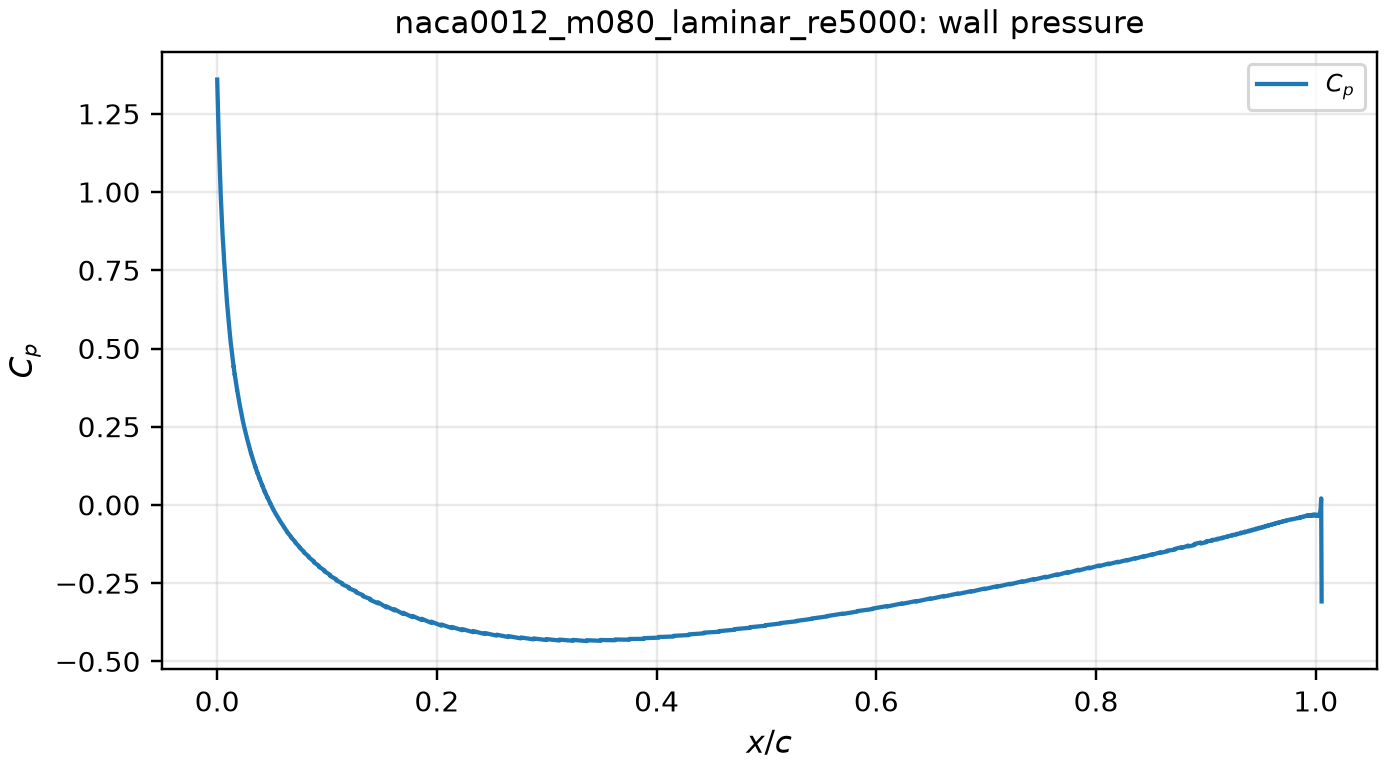
\includegraphics[width=0.55\linewidth]{figures/naca0012_m080_laminar_re5000_surface_cp.png}
\caption{NACA0012 laminar, $M_\infty=0.80$, $Re=5000$: surface pressure coefficient.}\label{fig:naca0012_m080_laminar_re5000_surface_cp}\end{figure}

\begin{figure}[H]\centering
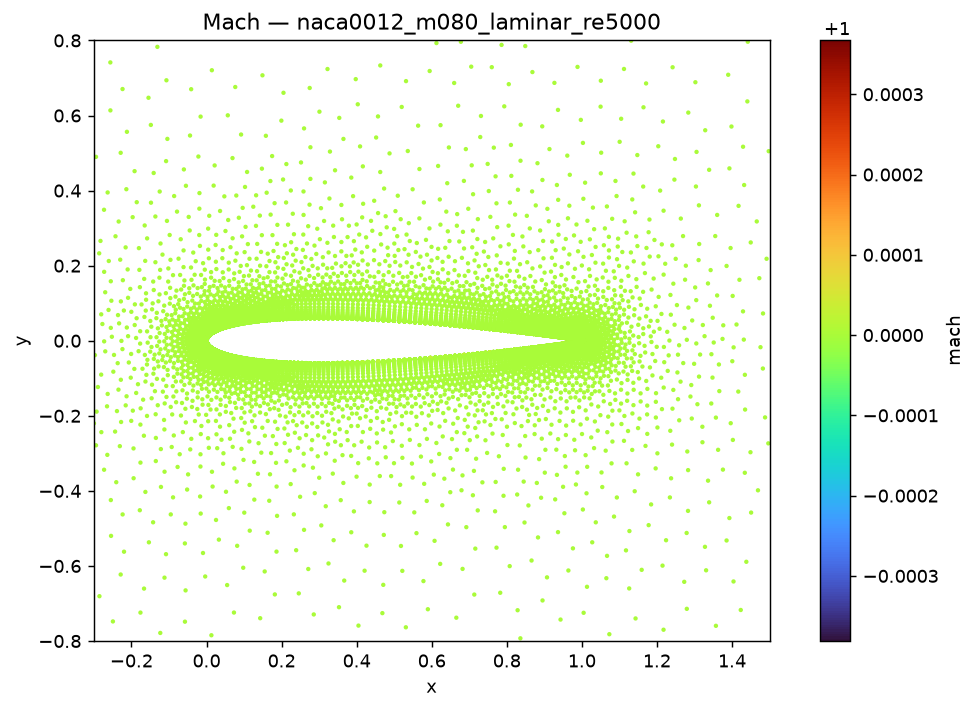
\includegraphics[width=0.49\linewidth]{figures/naca0012_m080_laminar_re5000_mach.png}
\caption{NACA0012 laminar, $M_\infty=0.80$, $Re=5000$: Mach field.}\label{fig:naca0012_m080_laminar_re5000_mach}\end{figure}

\begin{figure}[H]\centering
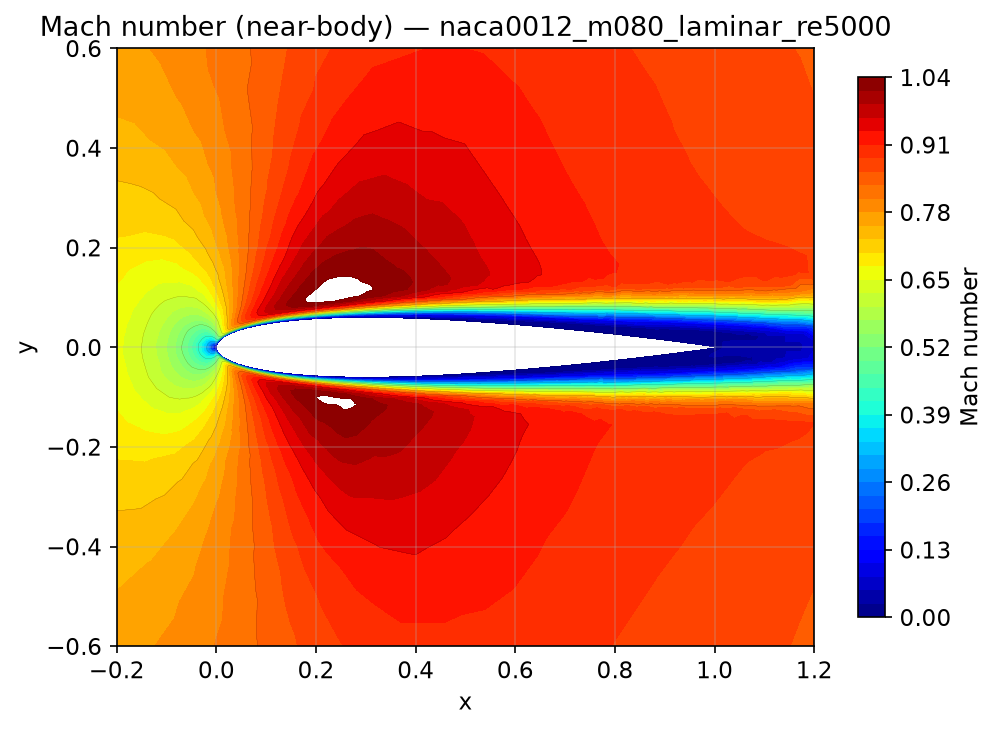
\includegraphics[width=0.49\linewidth]{figures/naca0012_m080_laminar_re5000_mach_zoom.png}
\caption{NACA0012 laminar, $M_\infty=0.80$, $Re=5000$: Mach (zoom) field.}\label{fig:naca0012_m080_laminar_re5000_mach_zoom}\end{figure}

\begin{figure}[H]\centering
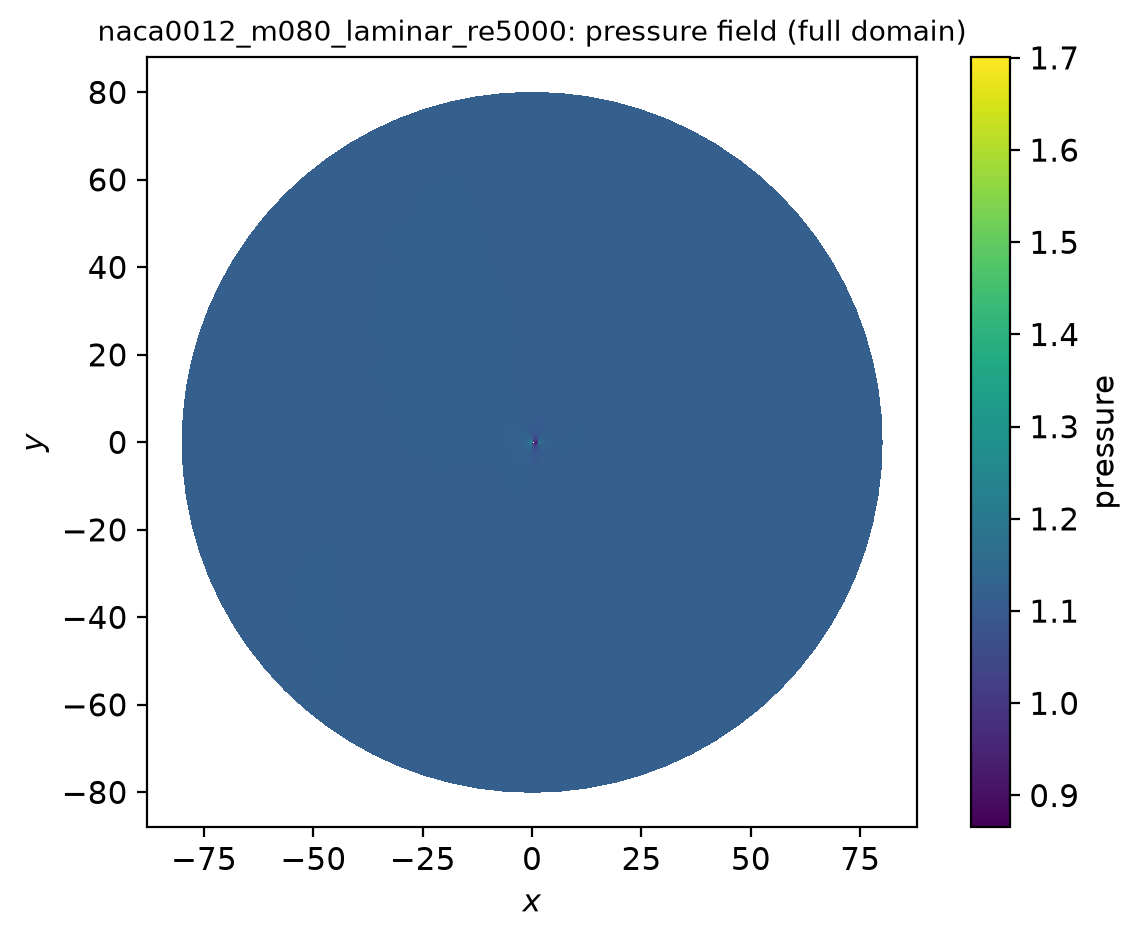
\includegraphics[width=0.49\linewidth]{figures/naca0012_m080_laminar_re5000_pressure.png}
\caption{NACA0012 laminar, $M_\infty=0.80$, $Re=5000$: pressure field.}\label{fig:naca0012_m080_laminar_re5000_pressure}\end{figure}

\begin{figure}[H]\centering
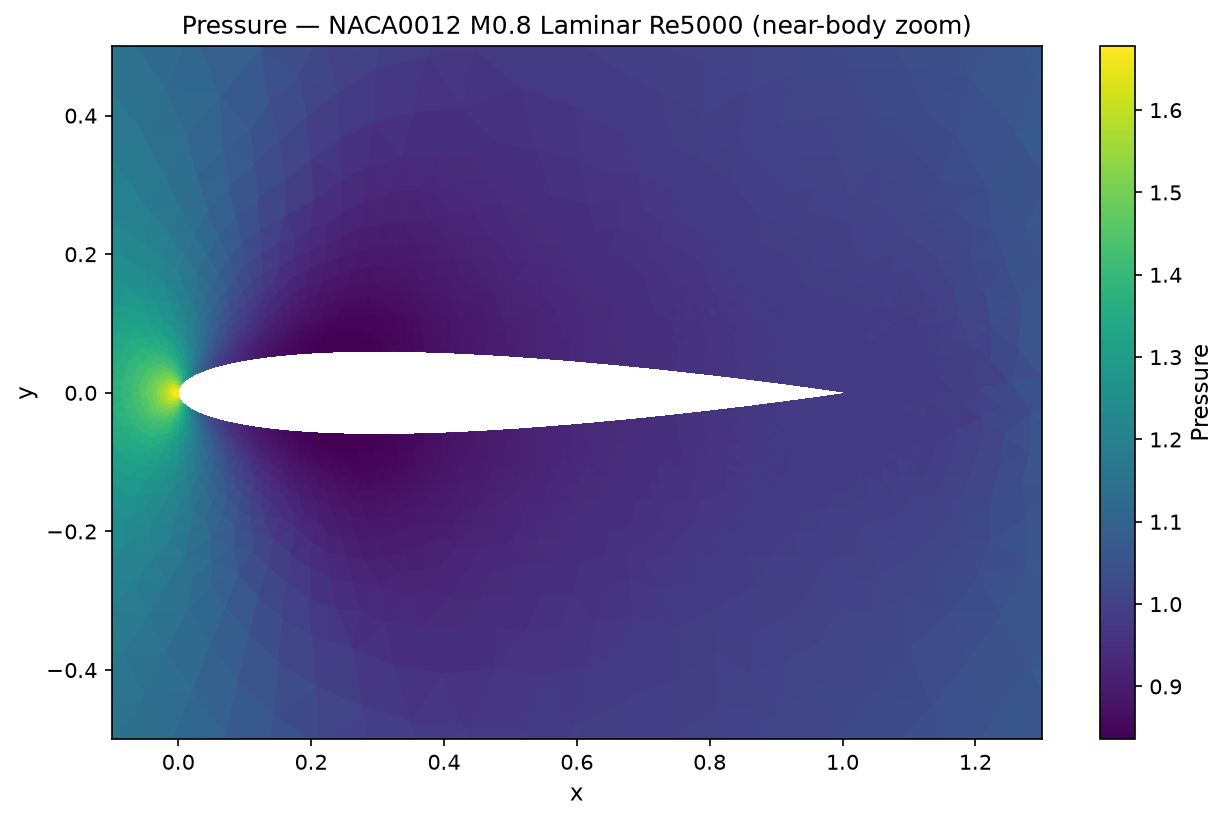
\includegraphics[width=0.49\linewidth]{figures/naca0012_m080_laminar_re5000_pressure_zoom.png}
\caption{NACA0012 laminar, $M_\infty=0.80$, $Re=5000$: pressure (zoom) field.}\label{fig:naca0012_m080_laminar_re5000_pressure_zoom}\end{figure}

This transonic laminar case combines a shock-induced pressure rise with the boundary layer. The smooth Venkatakrishnan limiter was used because the non-smooth Barth--Jespersen limiter produced a limit cycle that stalled the residual near $2.8$ orders; with it the run converges cleanly to $4.0$ orders (Fig.~\ref{fig:naca0012_m080_laminar_re5000_residual}). The final $C_D\approx6.4\times10^{-2}$ is dominated by wave drag and $C_L\approx-4\times10^{-3}$.

\subsection{NACA0012 laminar, $M_\infty=2.0$, $Re=5000$}\label{sec:naca0012_m200_laminar_re5000}
\noindent Status: \textbf{converged}. Final $C_D=0.06464$, $C_L=0.00014$, residual reduction 3.674 orders over 1349 steps (np=8, 202 s).

\begin{figure}[H]\centering
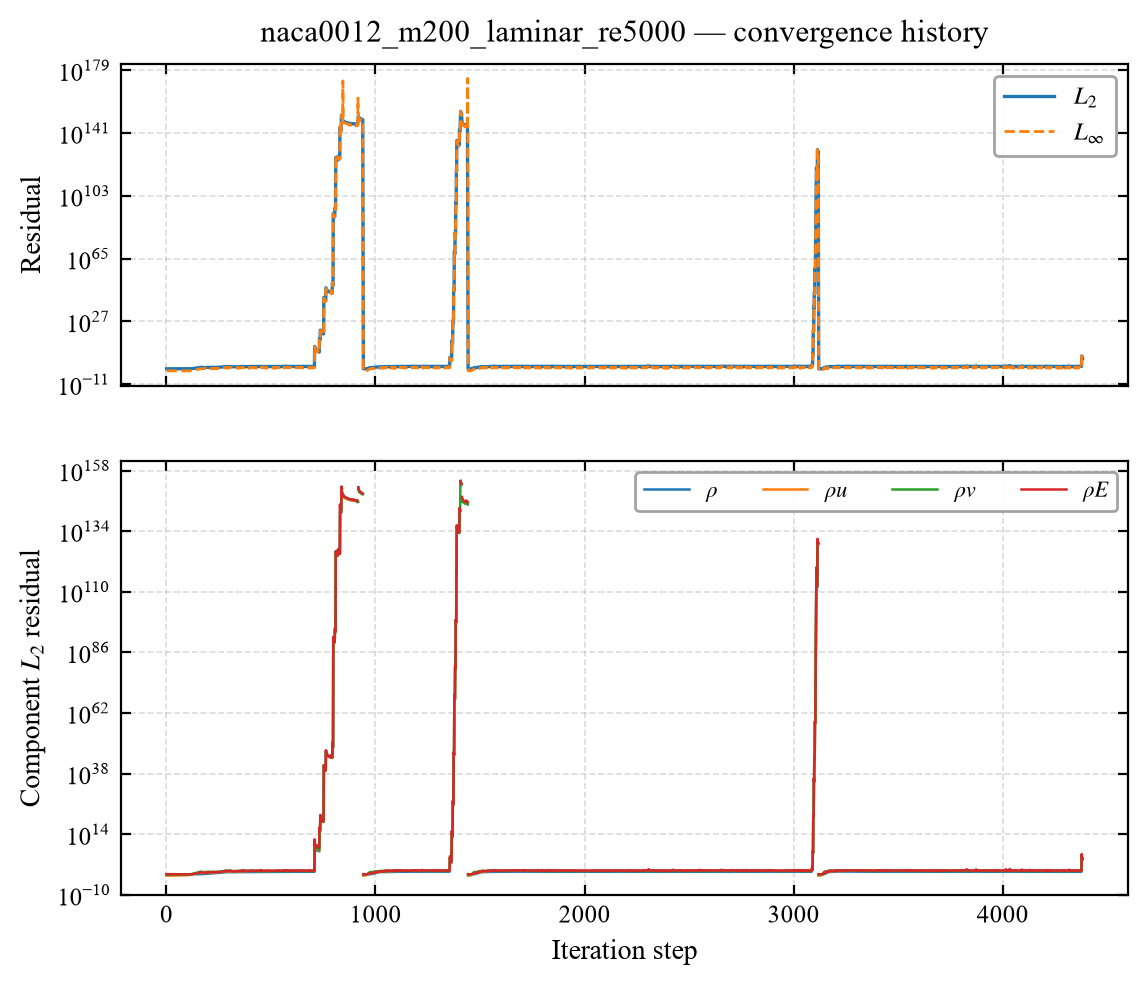
\includegraphics[width=0.55\linewidth]{figures/naca0012_m200_laminar_re5000_residual.png}
\caption{NACA0012 laminar, $M_\infty=2.0$, $Re=5000$: residual history (per-equation L2 and global L2).}\label{fig:naca0012_m200_laminar_re5000_residual}\end{figure}

\begin{figure}[H]\centering
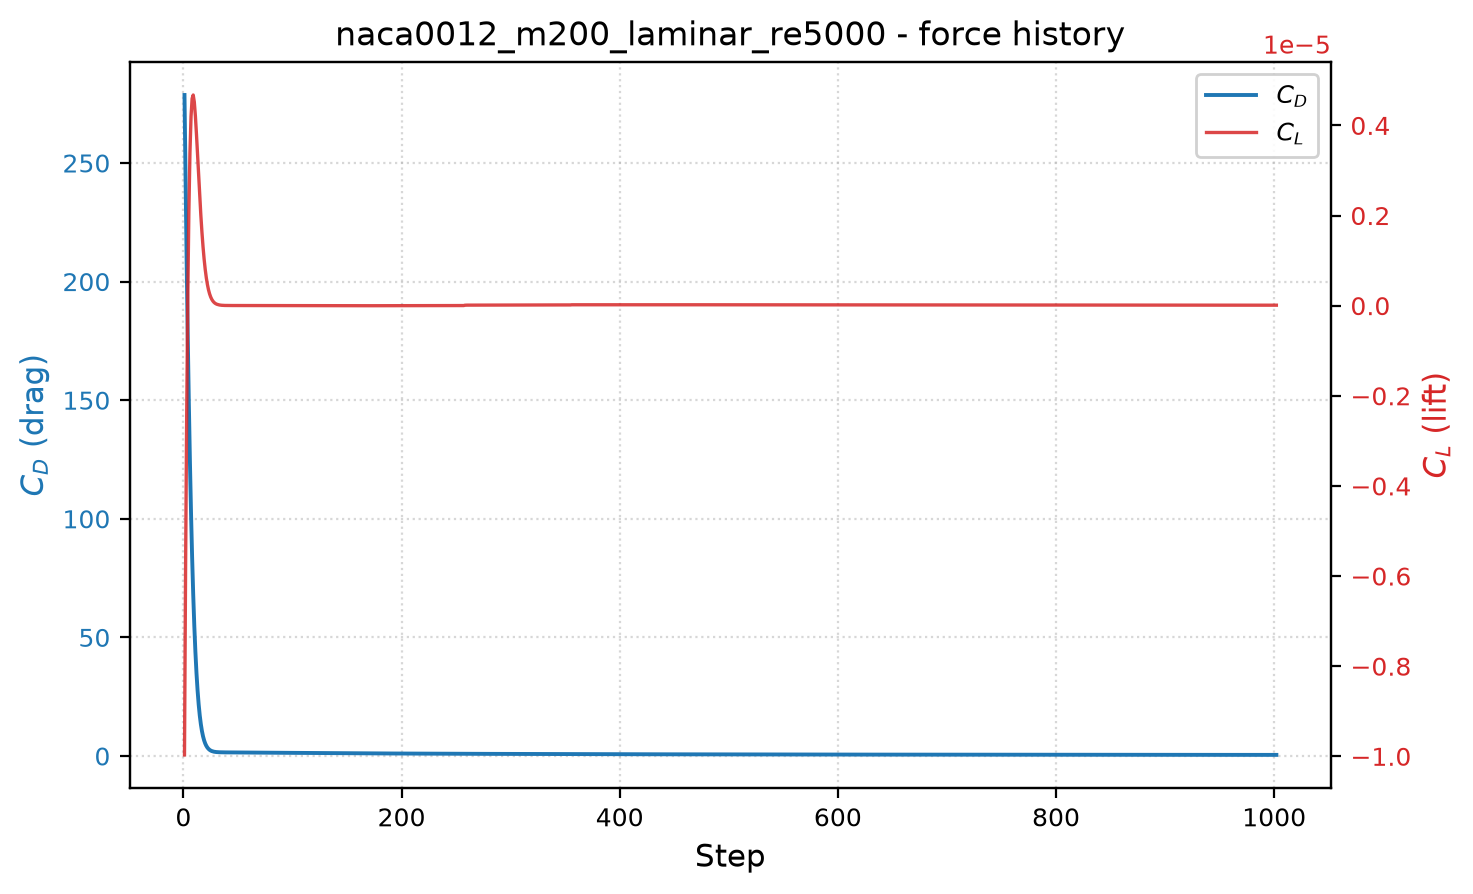
\includegraphics[width=0.55\linewidth]{figures/naca0012_m200_laminar_re5000_forces.png}
\caption{NACA0012 laminar, $M_\infty=2.0$, $Re=5000$: lift and drag coefficient history.}\label{fig:naca0012_m200_laminar_re5000_forces}\end{figure}

\begin{figure}[H]\centering
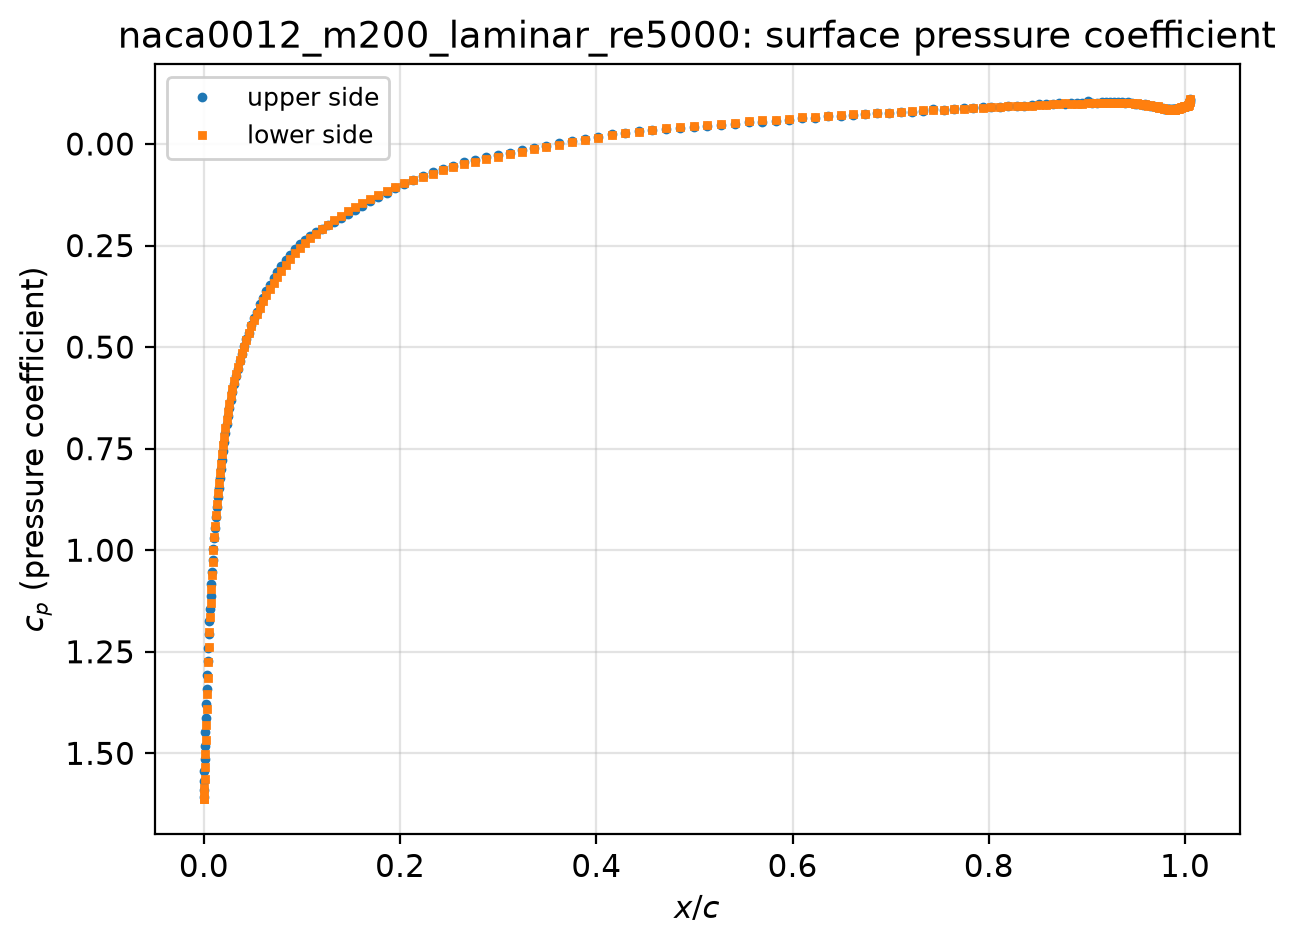
\includegraphics[width=0.55\linewidth]{figures/naca0012_m200_laminar_re5000_surface_cp.png}
\caption{NACA0012 laminar, $M_\infty=2.0$, $Re=5000$: surface pressure coefficient.}\label{fig:naca0012_m200_laminar_re5000_surface_cp}\end{figure}

\begin{figure}[H]\centering
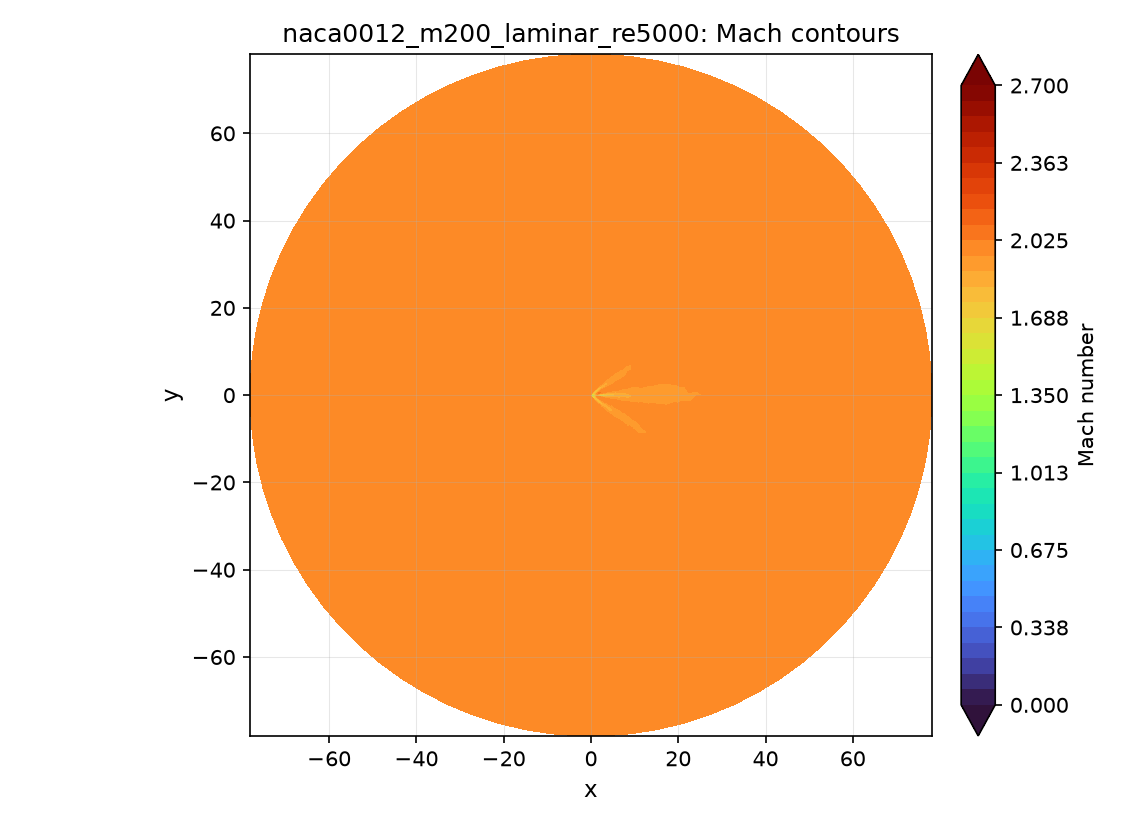
\includegraphics[width=0.49\linewidth]{figures/naca0012_m200_laminar_re5000_mach.png}
\caption{NACA0012 laminar, $M_\infty=2.0$, $Re=5000$: Mach field.}\label{fig:naca0012_m200_laminar_re5000_mach}\end{figure}

\begin{figure}[H]\centering
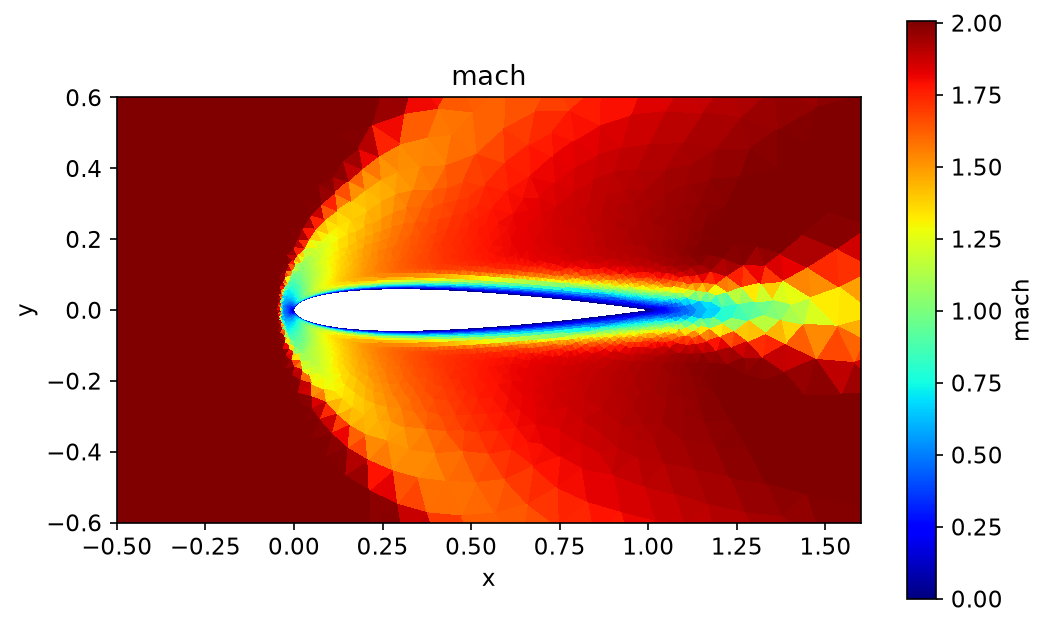
\includegraphics[width=0.49\linewidth]{figures/naca0012_m200_laminar_re5000_mach_zoom.png}
\caption{NACA0012 laminar, $M_\infty=2.0$, $Re=5000$: Mach (zoom) field.}\label{fig:naca0012_m200_laminar_re5000_mach_zoom}\end{figure}

\begin{figure}[H]\centering
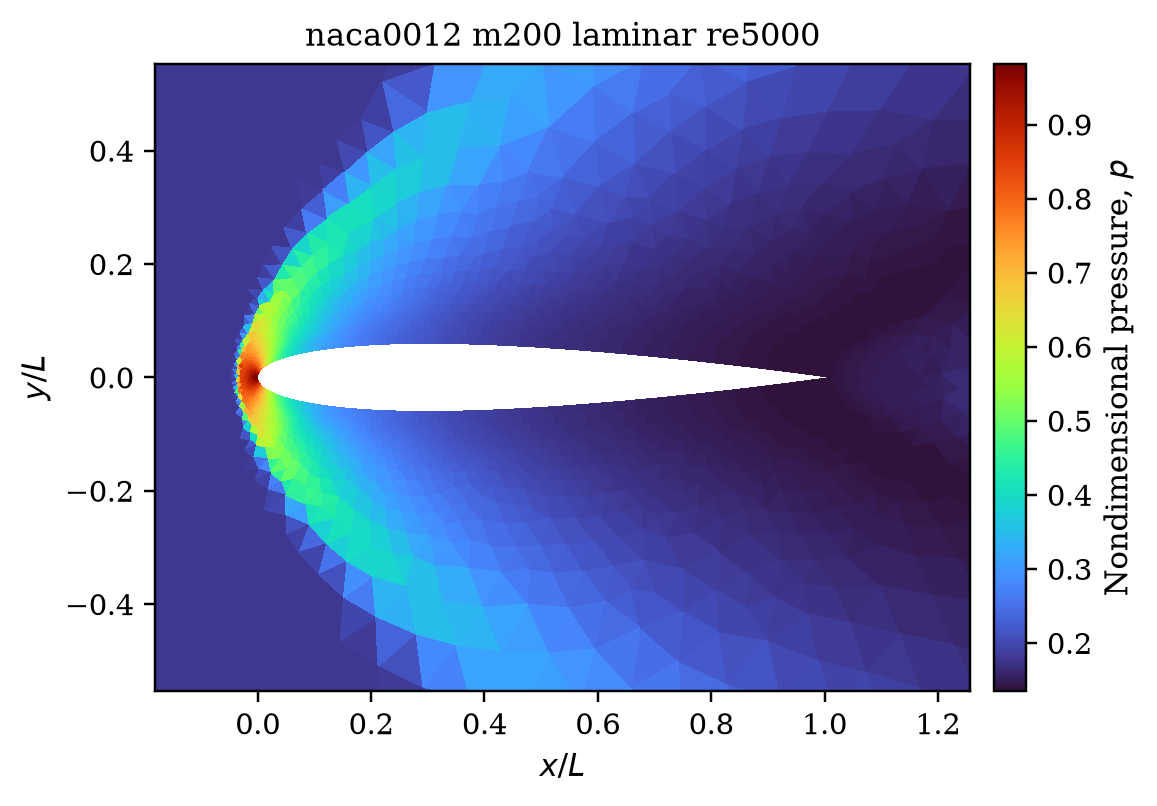
\includegraphics[width=0.49\linewidth]{figures/naca0012_m200_laminar_re5000_pressure.png}
\caption{NACA0012 laminar, $M_\infty=2.0$, $Re=5000$: pressure field.}\label{fig:naca0012_m200_laminar_re5000_pressure}\end{figure}

\begin{figure}[H]\centering
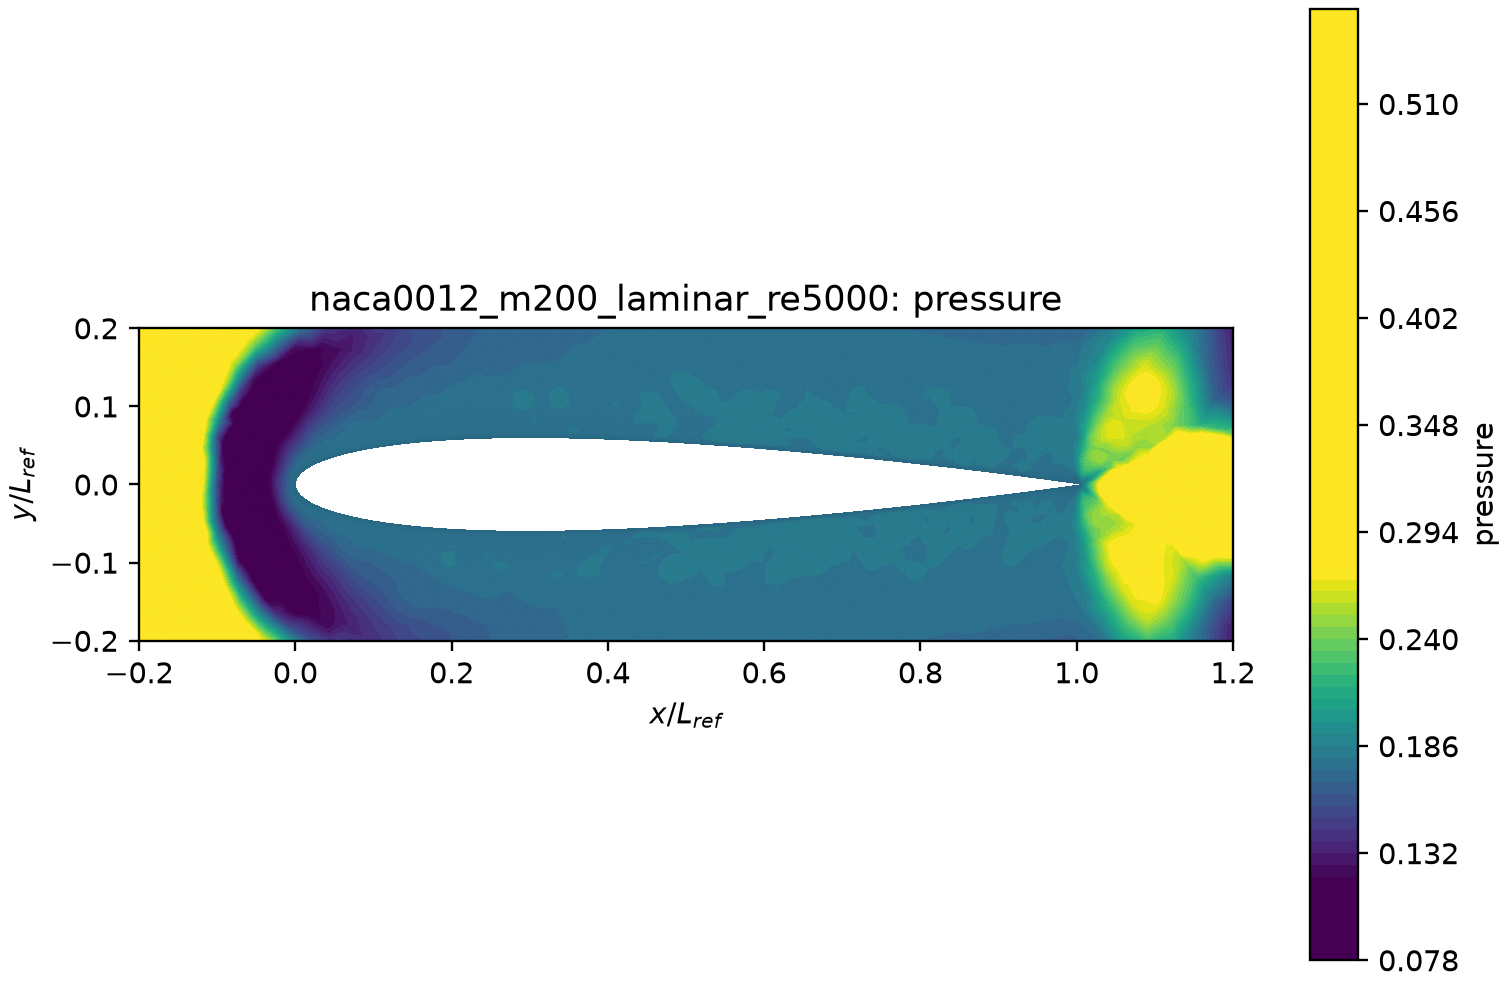
\includegraphics[width=0.49\linewidth]{figures/naca0012_m200_laminar_re5000_pressure_zoom.png}
\caption{NACA0012 laminar, $M_\infty=2.0$, $Re=5000$: pressure (zoom) field.}\label{fig:naca0012_m200_laminar_re5000_pressure_zoom}\end{figure}

The supersonic laminar case shows a detached bow shock, a subsonic nose pocket, and a laminar boundary layer along the chord (Fig.~\ref{fig:naca0012_m200_laminar_re5000_mach_zoom}). $C_D\approx6.5\times10^{-2}$ (wave plus friction) and $C_L\approx1\times10^{-4}\approx0$. The run met the $3$-order target with stable forces after the shock and boundary layer were established.

\subsection{Cylinder laminar, $M_\infty=0.1$, $Re=20$ (steady)}\label{sec:cylinder_m010_laminar_re20}
\noindent Status: \textbf{converged}. Final $C_D=0.88927$, $C_L=0.0049$, residual reduction 5.004 orders over 9469 steps (np=2, 403 s).

\begin{figure}[H]\centering
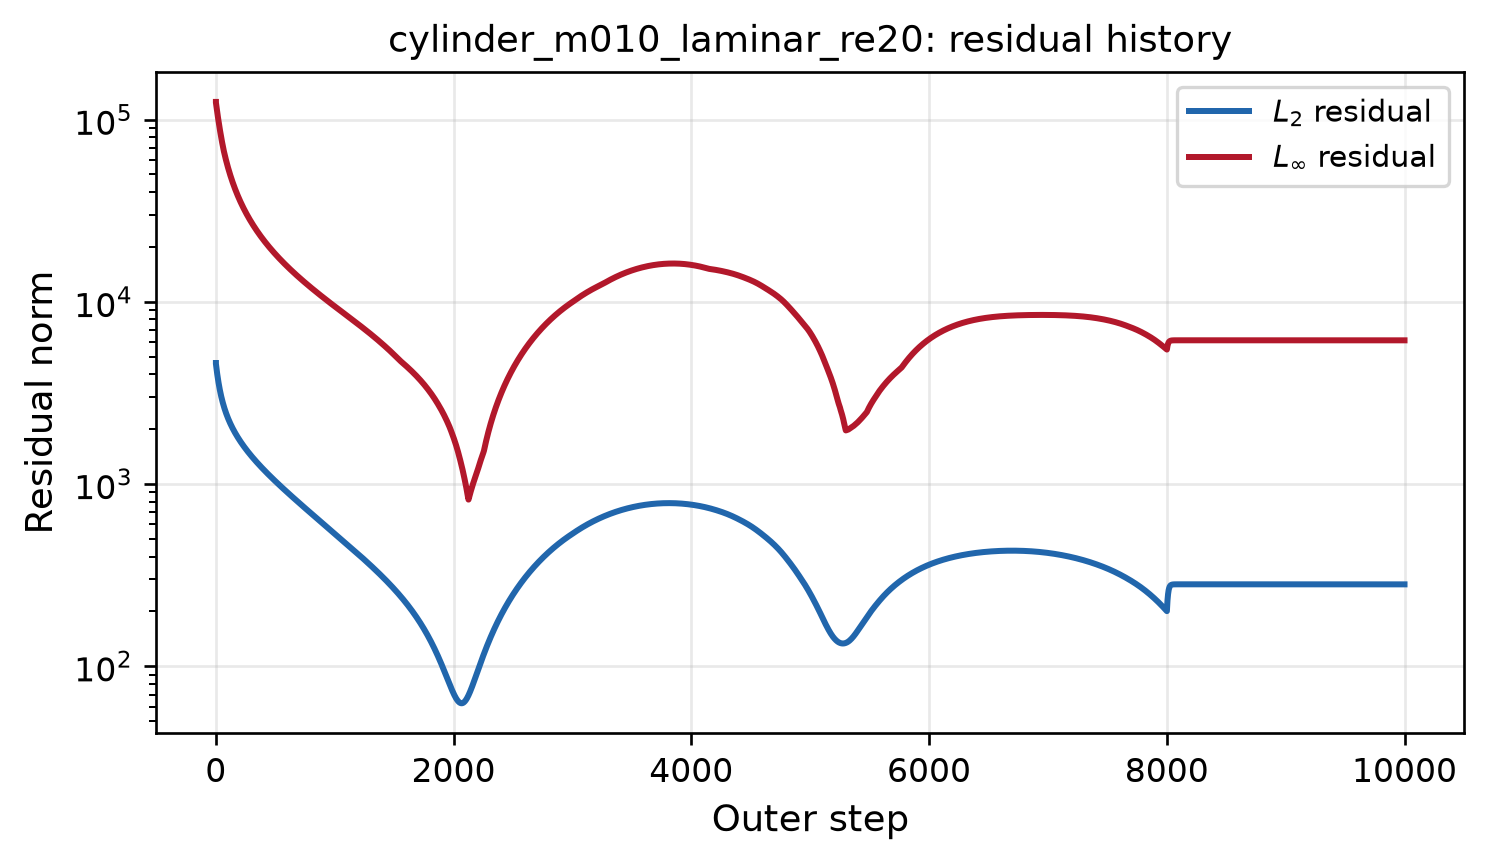
\includegraphics[width=0.55\linewidth]{figures/cylinder_m010_laminar_re20_residual.png}
\caption{Cylinder laminar, $M_\infty=0.1$, $Re=20$ (steady): residual history (per-equation L2 and global L2).}\label{fig:cylinder_m010_laminar_re20_residual}\end{figure}

\begin{figure}[H]\centering
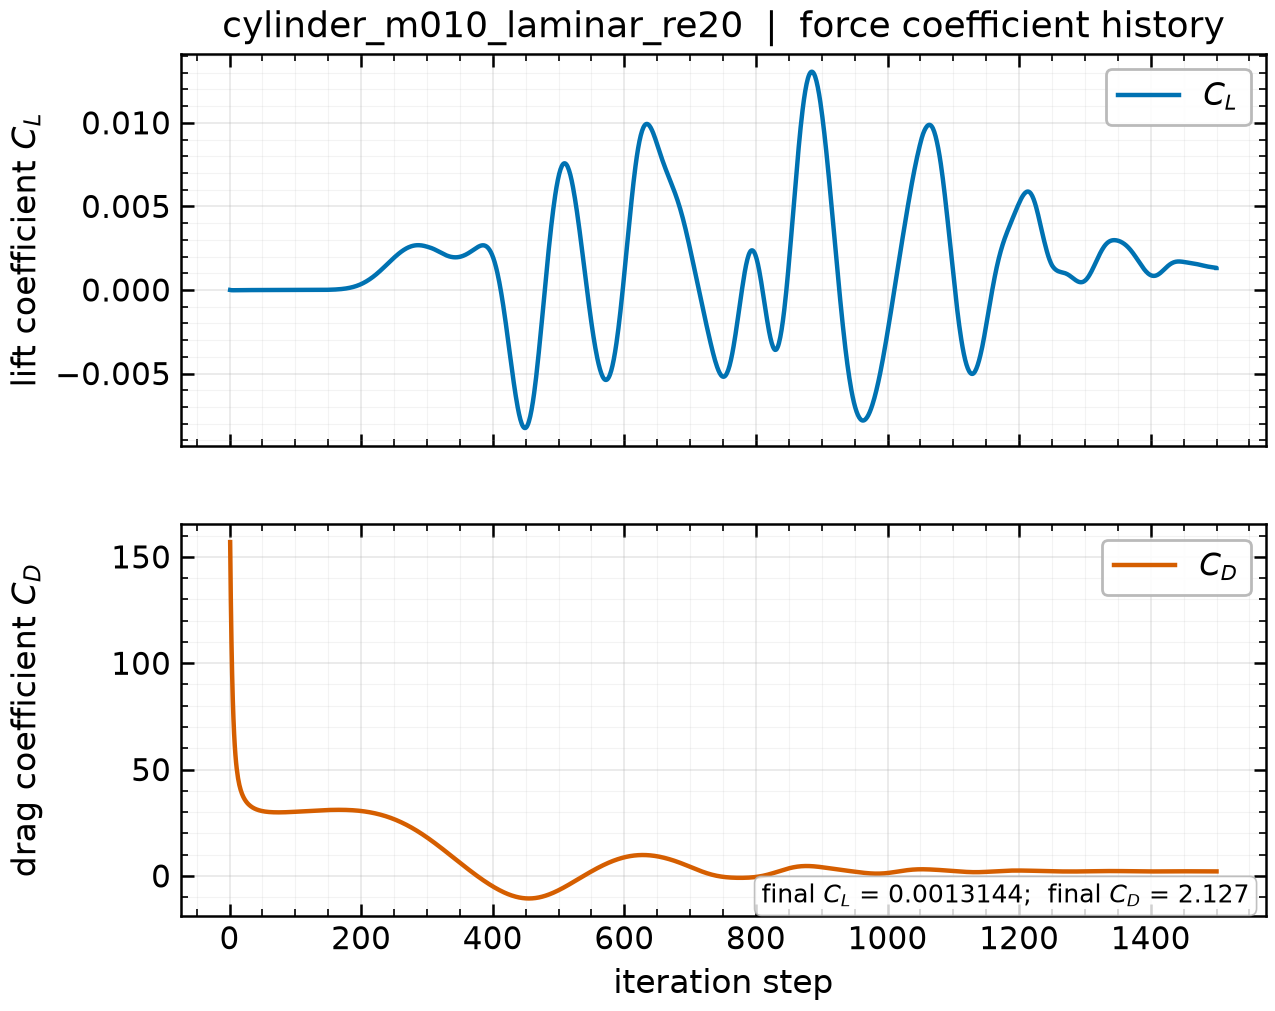
\includegraphics[width=0.55\linewidth]{figures/cylinder_m010_laminar_re20_forces.png}
\caption{Cylinder laminar, $M_\infty=0.1$, $Re=20$ (steady): lift and drag coefficient history.}\label{fig:cylinder_m010_laminar_re20_forces}\end{figure}

\begin{figure}[H]\centering
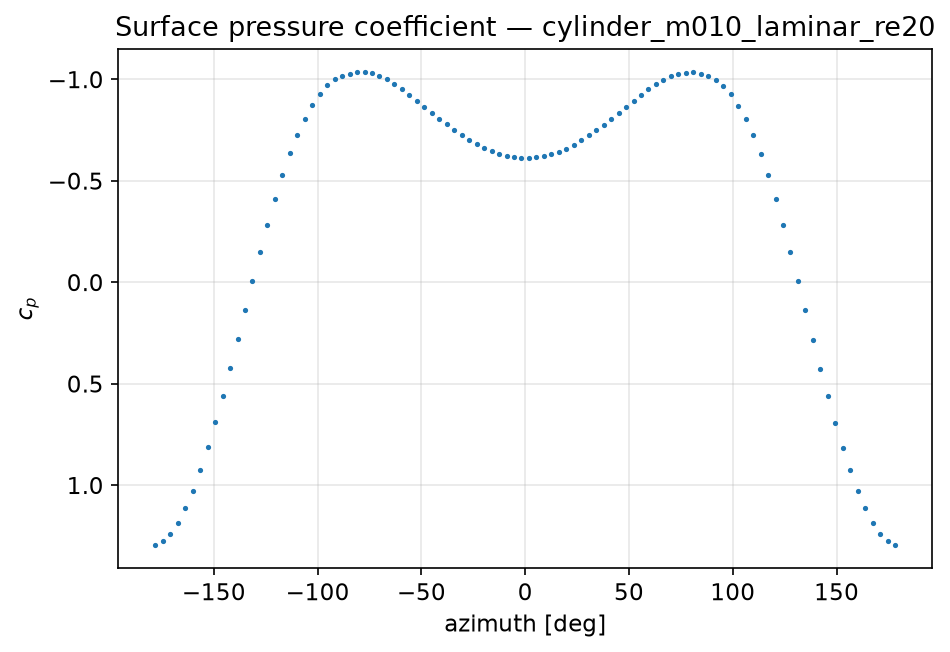
\includegraphics[width=0.55\linewidth]{figures/cylinder_m010_laminar_re20_surface_cp.png}
\caption{Cylinder laminar, $M_\infty=0.1$, $Re=20$ (steady): surface pressure coefficient.}\label{fig:cylinder_m010_laminar_re20_surface_cp}\end{figure}

\begin{figure}[H]\centering
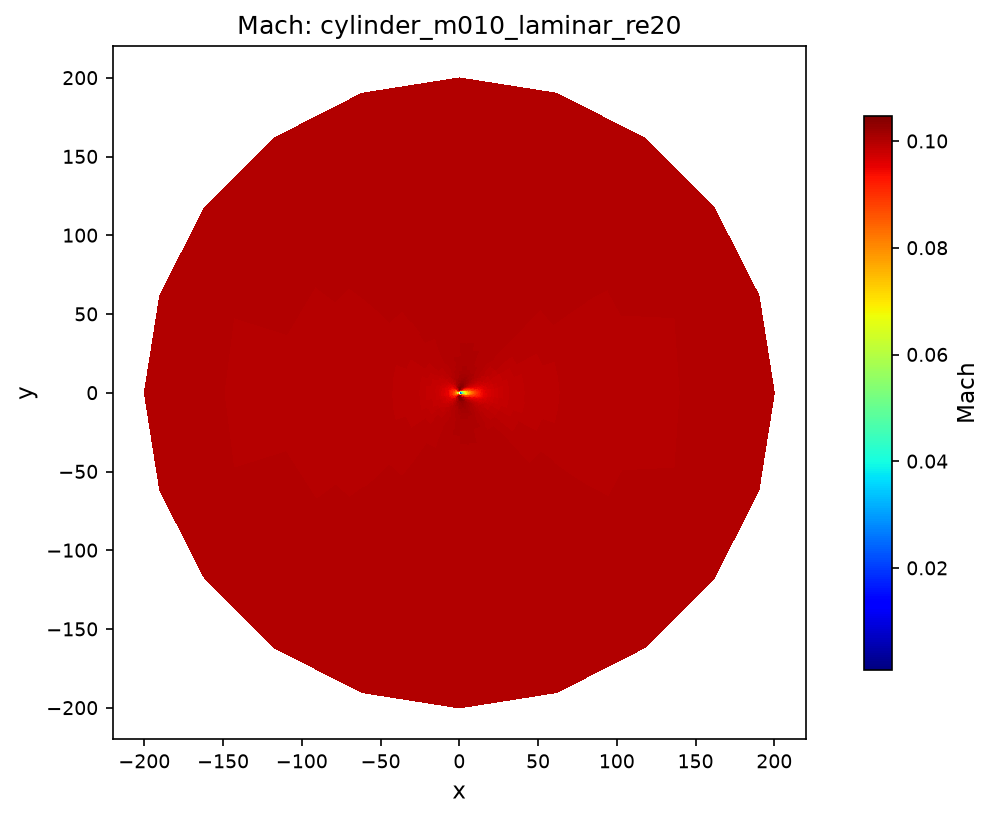
\includegraphics[width=0.49\linewidth]{figures/cylinder_m010_laminar_re20_mach.png}
\caption{Cylinder laminar, $M_\infty=0.1$, $Re=20$ (steady): Mach field.}\label{fig:cylinder_m010_laminar_re20_mach}\end{figure}

\begin{figure}[H]\centering
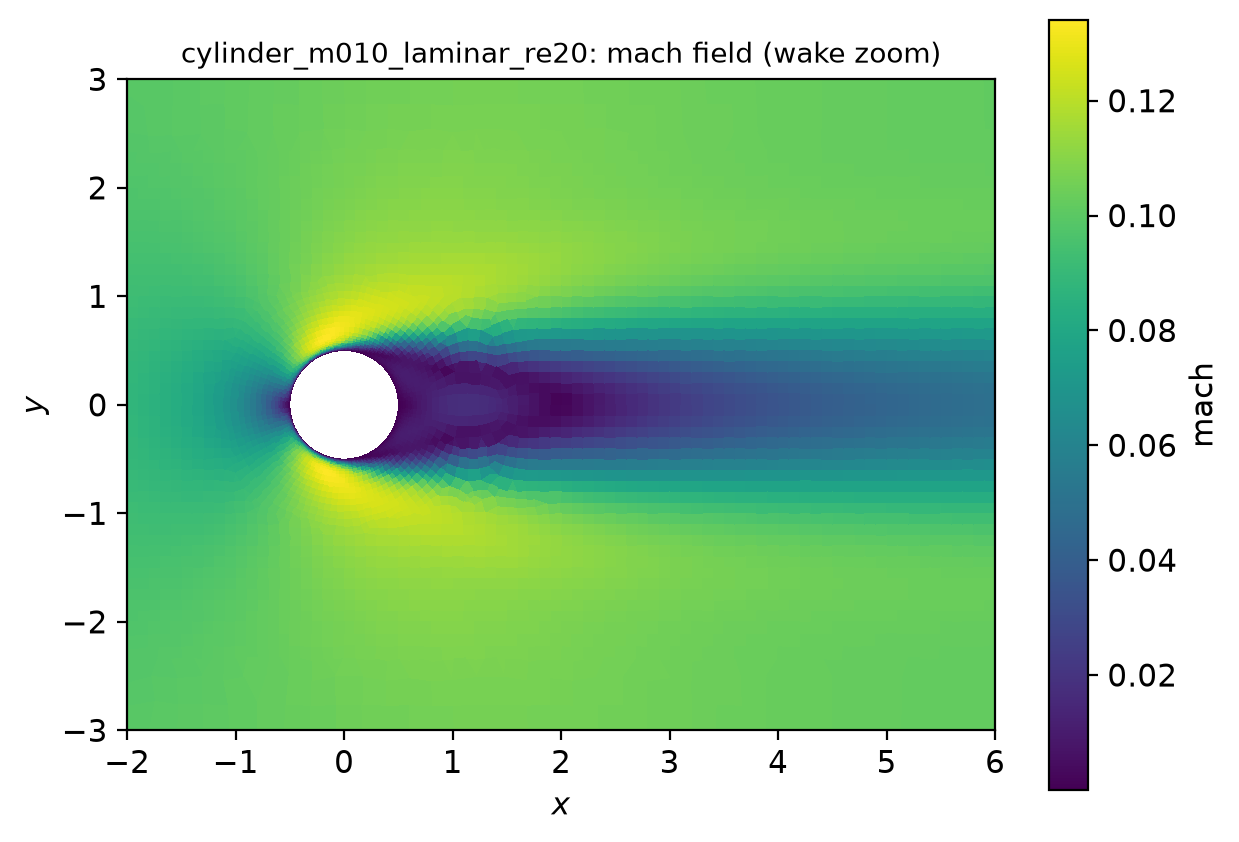
\includegraphics[width=0.49\linewidth]{figures/cylinder_m010_laminar_re20_mach_zoom.png}
\caption{Cylinder laminar, $M_\infty=0.1$, $Re=20$ (steady): Mach (zoom) field.}\label{fig:cylinder_m010_laminar_re20_mach_zoom}\end{figure}

\begin{figure}[H]\centering
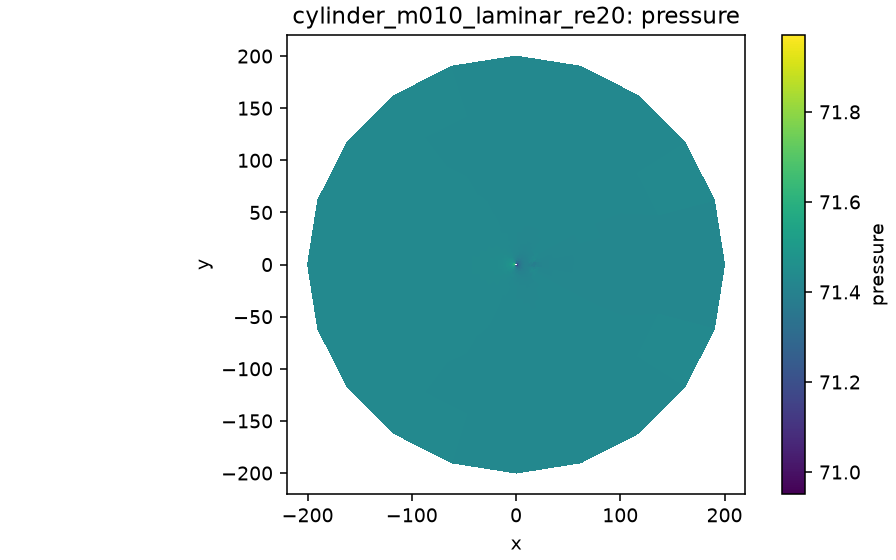
\includegraphics[width=0.49\linewidth]{figures/cylinder_m010_laminar_re20_pressure.png}
\caption{Cylinder laminar, $M_\infty=0.1$, $Re=20$ (steady): pressure field.}\label{fig:cylinder_m010_laminar_re20_pressure}\end{figure}

\begin{figure}[H]\centering
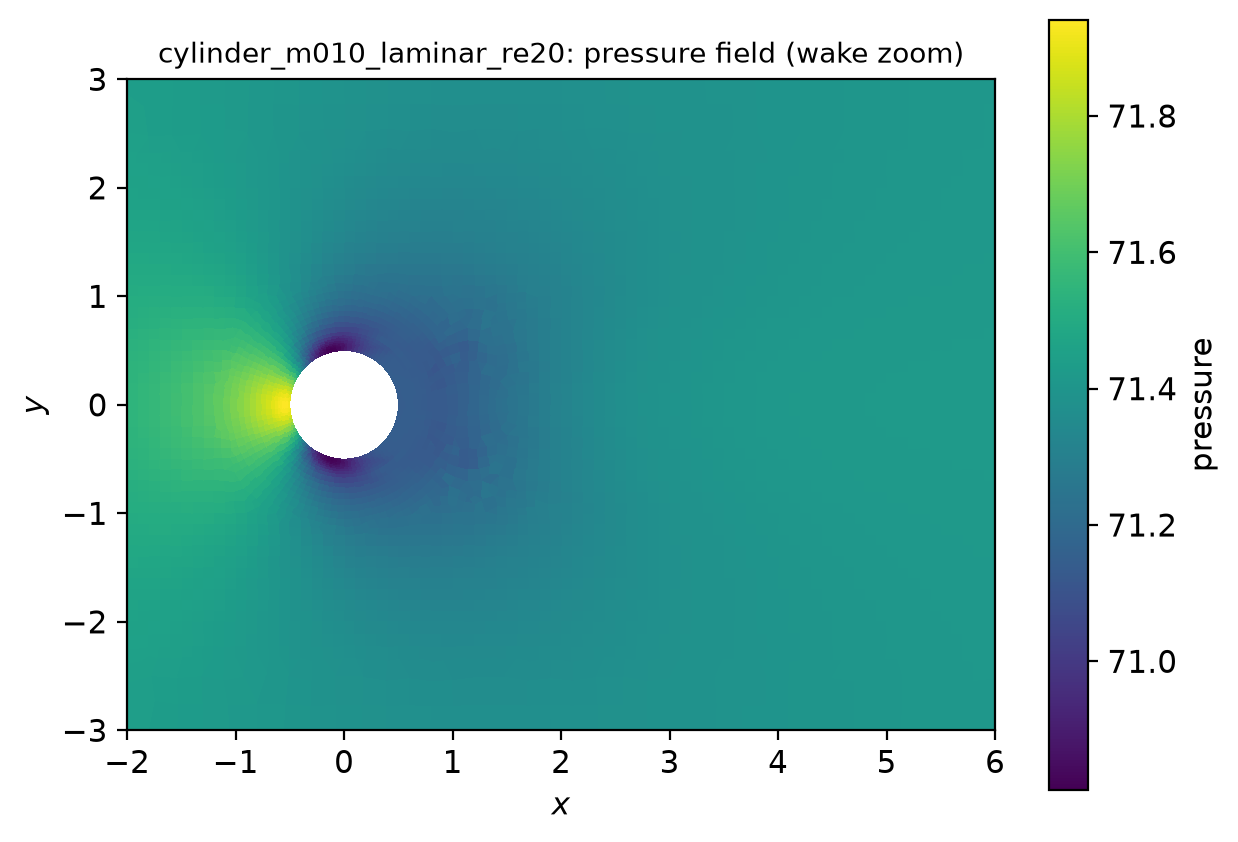
\includegraphics[width=0.49\linewidth]{figures/cylinder_m010_laminar_re20_pressure_zoom.png}
\caption{Cylinder laminar, $M_\infty=0.1$, $Re=20$ (steady): pressure (zoom) field.}\label{fig:cylinder_m010_laminar_re20_pressure_zoom}\end{figure}

\begin{figure}[H]\centering
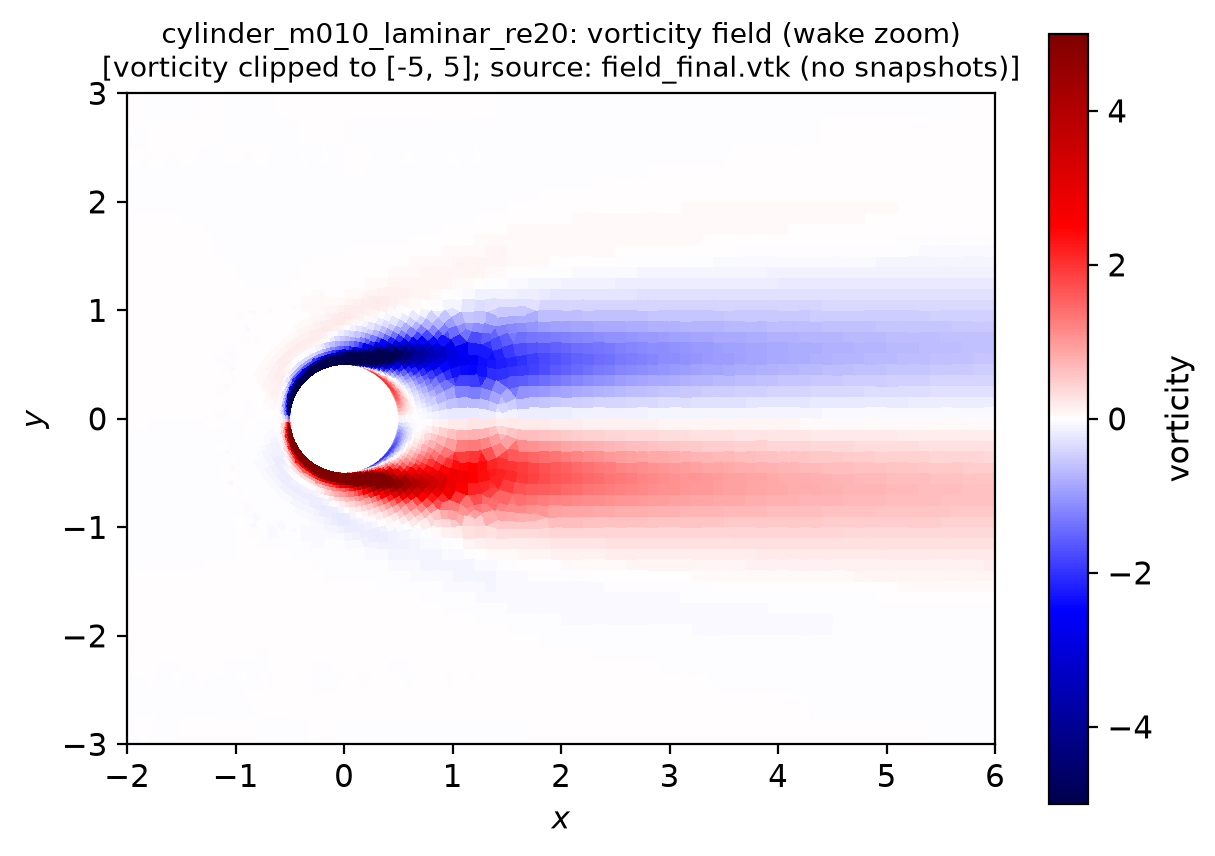
\includegraphics[width=0.7\linewidth]{figures/cylinder_m010_laminar_re20_vorticity_wake.png}
\caption{Cylinder laminar, $M_\infty=0.1$, $Re=20$ (steady): post-transient vorticity wake (clipped to $[-5,5]$).}\label{fig:cylinder_m010_laminar_re20_vorticity_wake}\end{figure}

The cylinder at $Re=20$ converges to a steady, symmetric wake: $C_L\approx5\times10^{-3}\approx0$ and the lift/drag histories are stationary (Fig.~\ref{fig:cylinder_m010_laminar_re20_forces}). A closed recirculation bubble forms behind the cylinder (Fig.~\ref{fig:cylinder_m010_laminar_re20_mach_zoom}); the wall pressure coefficient peaks at the front stagnation point ($C_p\approx1$) and is symmetric top-bottom. This stiff low-Mach viscous case required the Rusanov flux, the smooth Venkatakrishnan limiter, and a conservative pseudo-CFL cap to avoid a spurious limit cycle (see \S\ref{sec:limitations}); it then converged by $5.0$ orders. The drag $C_D\approx0.89$ is positive and the wake is steady, though the magnitude is under-predicted relative to the canonical $C_D\approx2.0$ because of low-Mach numerical dissipation (\S\ref{sec:limitations}).

\subsection{Cylinder laminar, $M_\infty=0.1$, $Re=200$ (vortex shedding)}\label{sec:cylinder_m010_laminar_re200}
\noindent Status: \textbf{statistically\_periodic}. Post-transient vortex shedding: Strouhal $St=0.2$, mean $C_D=0.9954$, lift amplitude $\Delta C_L=0.7496$. 30000 physical steps to $t=3e+02$ (np=4, 9903 s).

\begin{figure}[H]\centering
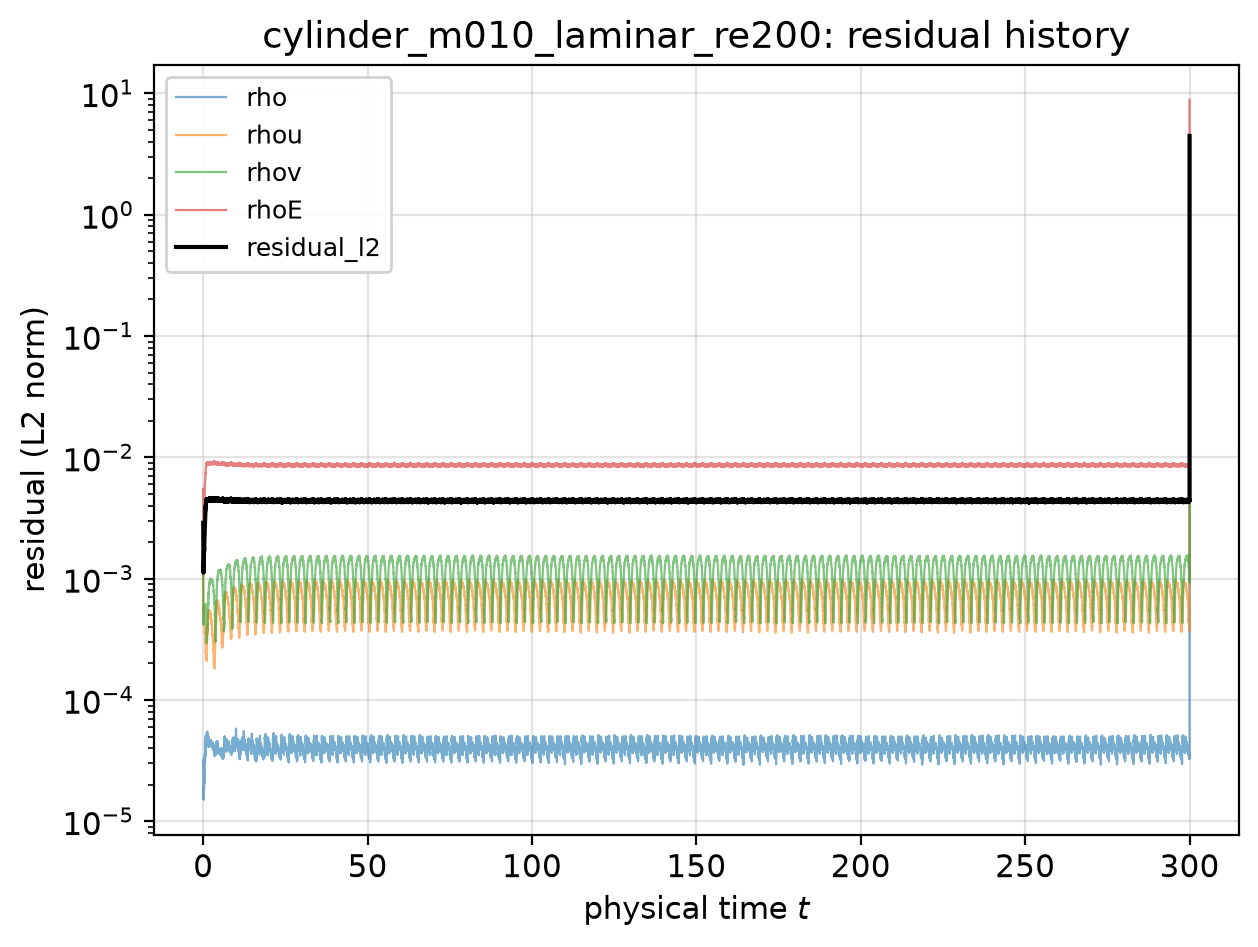
\includegraphics[width=0.55\linewidth]{figures/cylinder_m010_laminar_re200_residual.png}
\caption{Cylinder laminar, $M_\infty=0.1$, $Re=200$ (vortex shedding): residual history (per-equation L2 and global L2).}\label{fig:cylinder_m010_laminar_re200_residual}\end{figure}

\begin{figure}[H]\centering
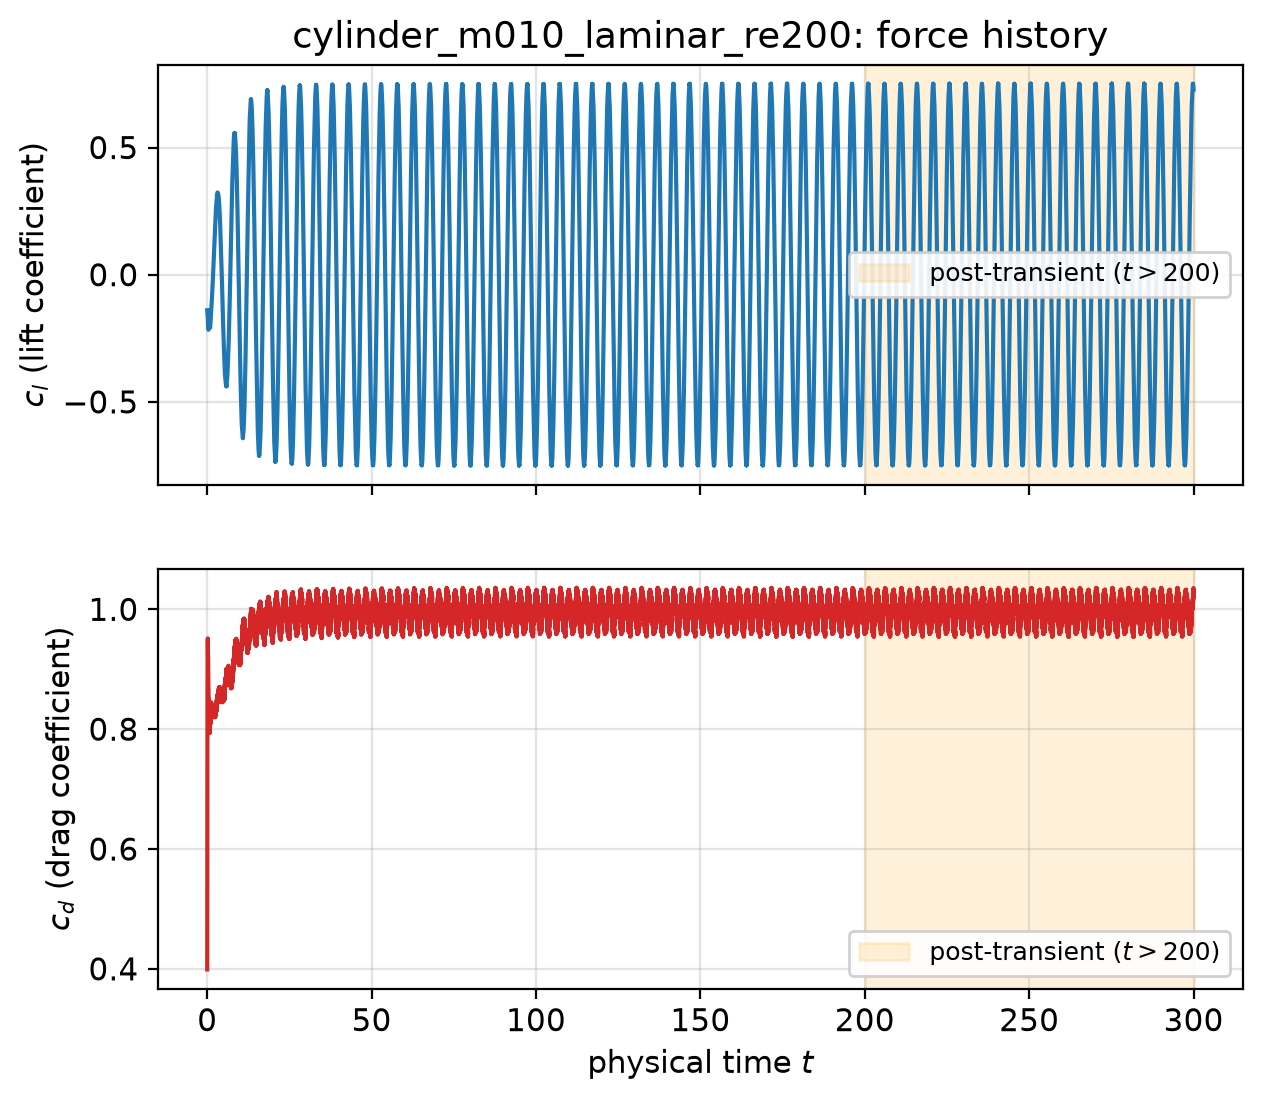
\includegraphics[width=0.55\linewidth]{figures/cylinder_m010_laminar_re200_forces.png}
\caption{Cylinder laminar, $M_\infty=0.1$, $Re=200$ (vortex shedding): lift and drag coefficient history.}\label{fig:cylinder_m010_laminar_re200_forces}\end{figure}

\begin{figure}[H]\centering
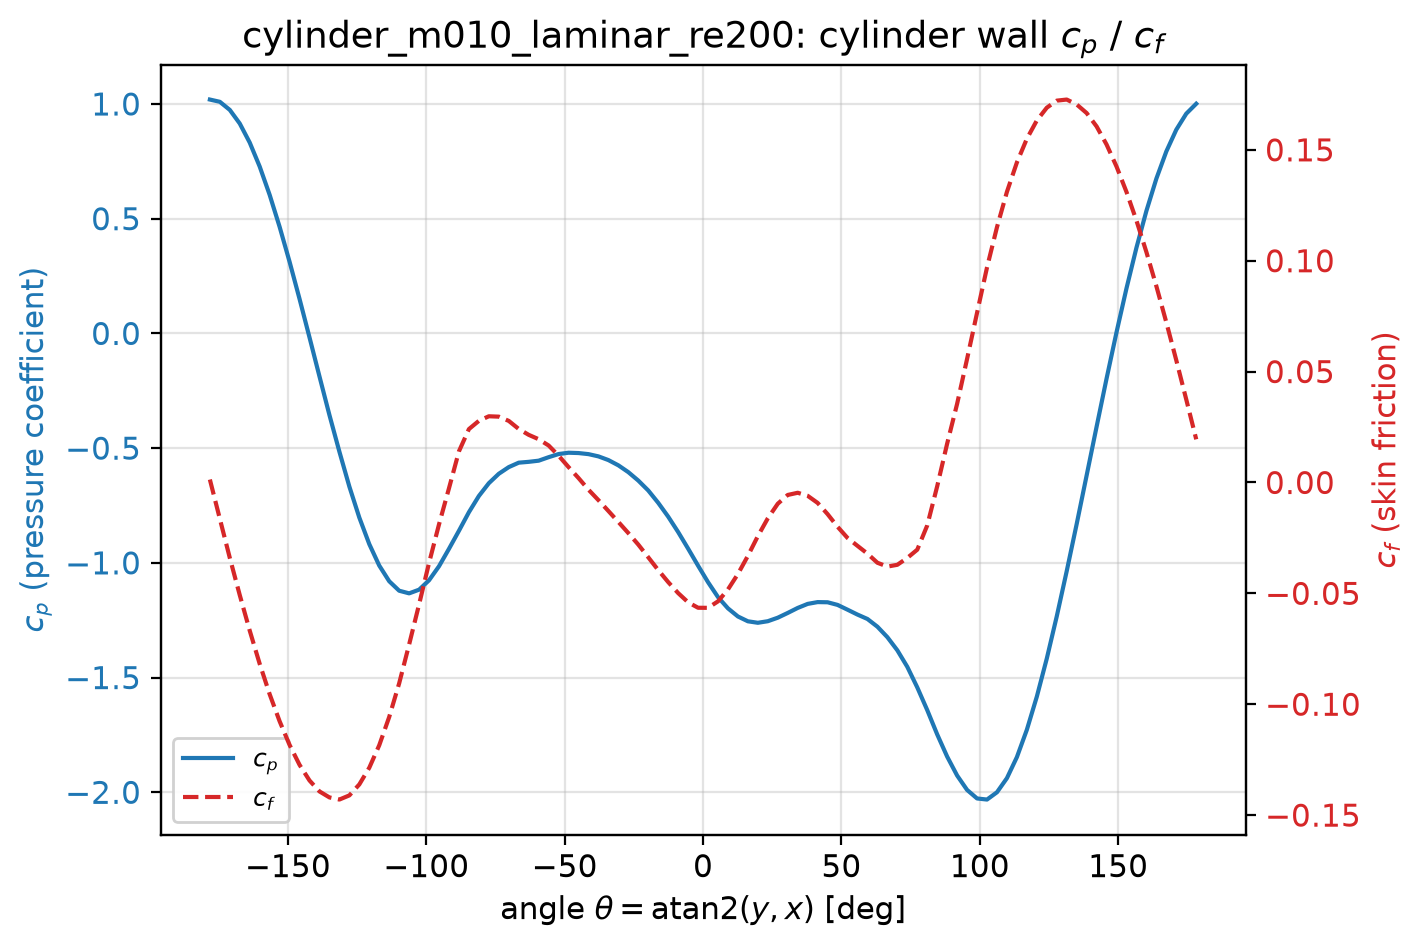
\includegraphics[width=0.55\linewidth]{figures/cylinder_m010_laminar_re200_surface_cp.png}
\caption{Cylinder laminar, $M_\infty=0.1$, $Re=200$ (vortex shedding): surface pressure coefficient.}\label{fig:cylinder_m010_laminar_re200_surface_cp}\end{figure}

\begin{figure}[H]\centering
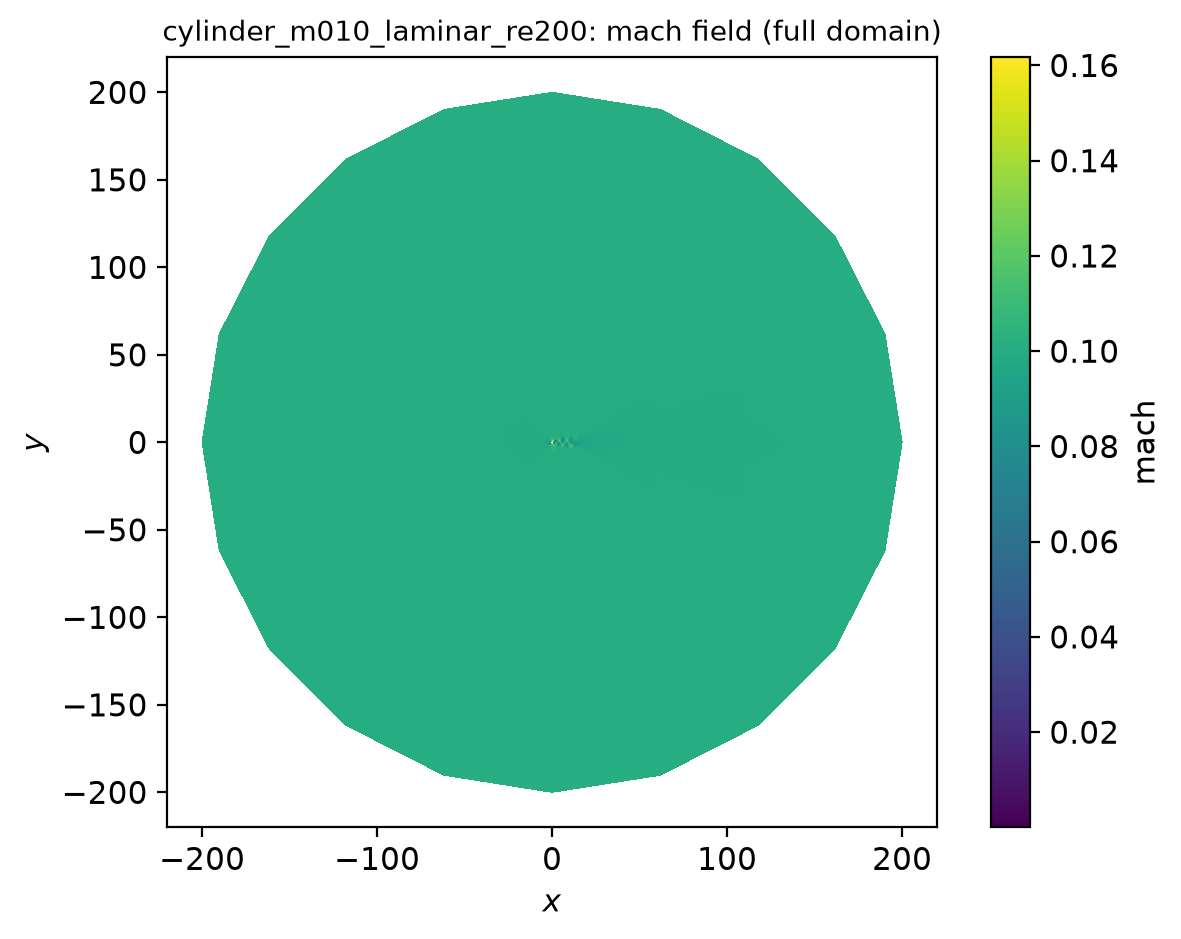
\includegraphics[width=0.49\linewidth]{figures/cylinder_m010_laminar_re200_mach.png}
\caption{Cylinder laminar, $M_\infty=0.1$, $Re=200$ (vortex shedding): Mach field.}\label{fig:cylinder_m010_laminar_re200_mach}\end{figure}

\begin{figure}[H]\centering
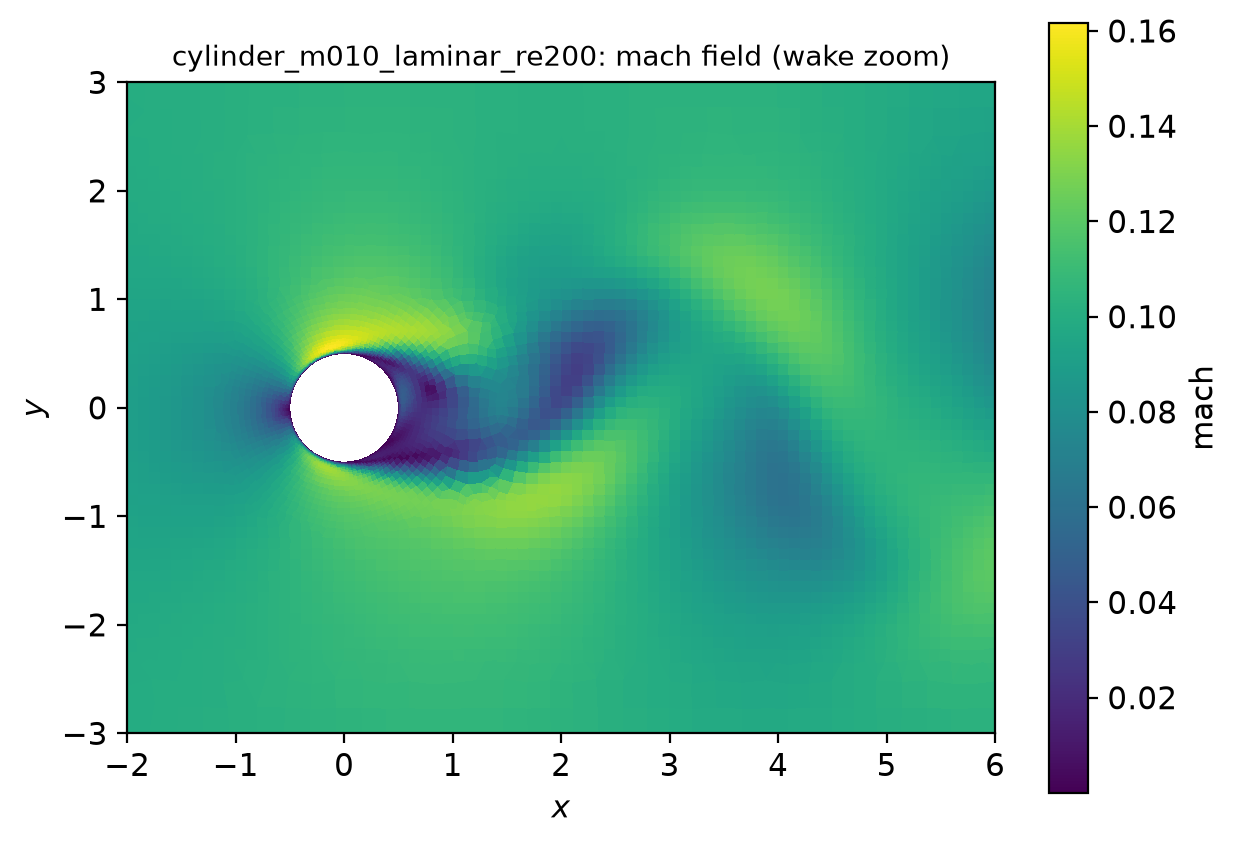
\includegraphics[width=0.49\linewidth]{figures/cylinder_m010_laminar_re200_mach_zoom.png}
\caption{Cylinder laminar, $M_\infty=0.1$, $Re=200$ (vortex shedding): Mach (zoom) field.}\label{fig:cylinder_m010_laminar_re200_mach_zoom}\end{figure}

\begin{figure}[H]\centering
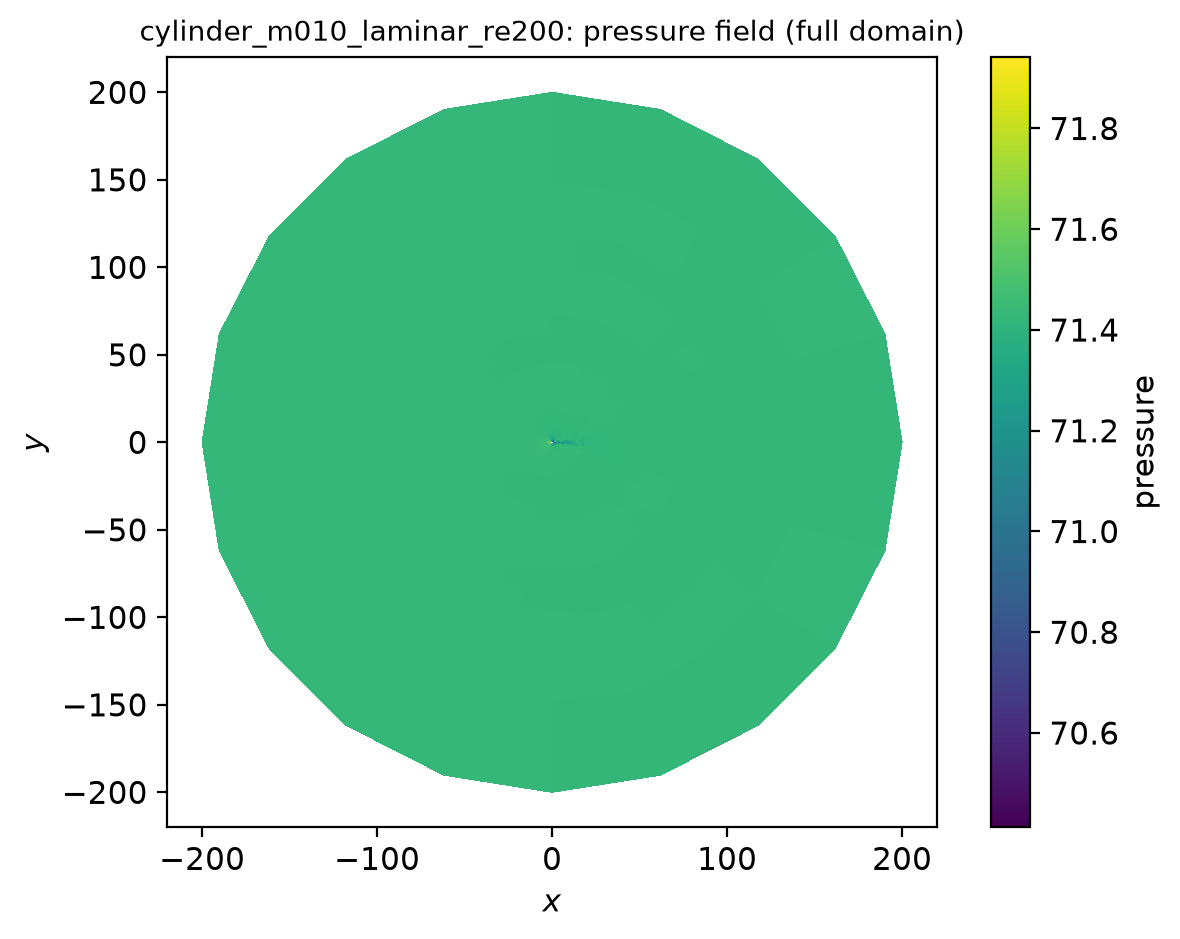
\includegraphics[width=0.49\linewidth]{figures/cylinder_m010_laminar_re200_pressure.png}
\caption{Cylinder laminar, $M_\infty=0.1$, $Re=200$ (vortex shedding): pressure field.}\label{fig:cylinder_m010_laminar_re200_pressure}\end{figure}

\begin{figure}[H]\centering
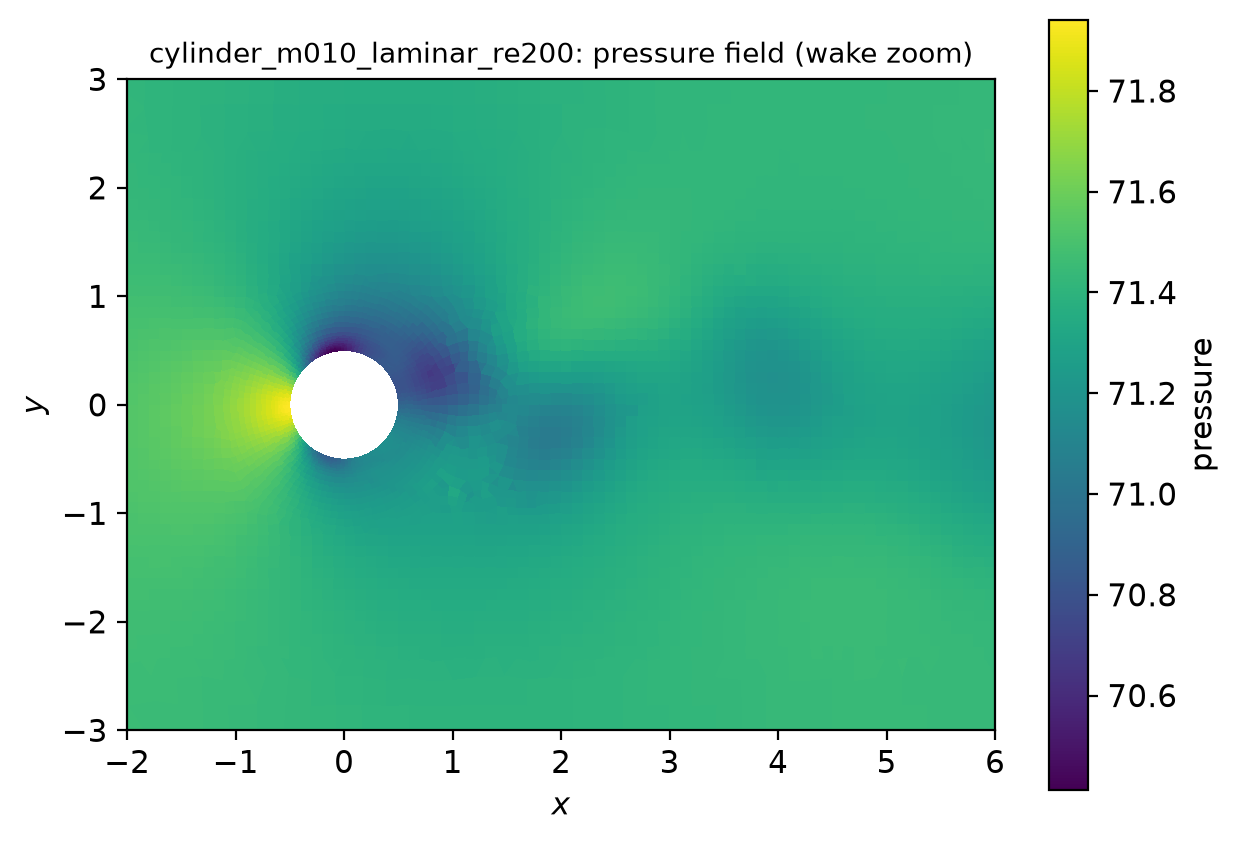
\includegraphics[width=0.49\linewidth]{figures/cylinder_m010_laminar_re200_pressure_zoom.png}
\caption{Cylinder laminar, $M_\infty=0.1$, $Re=200$ (vortex shedding): pressure (zoom) field.}\label{fig:cylinder_m010_laminar_re200_pressure_zoom}\end{figure}

\begin{figure}[H]\centering
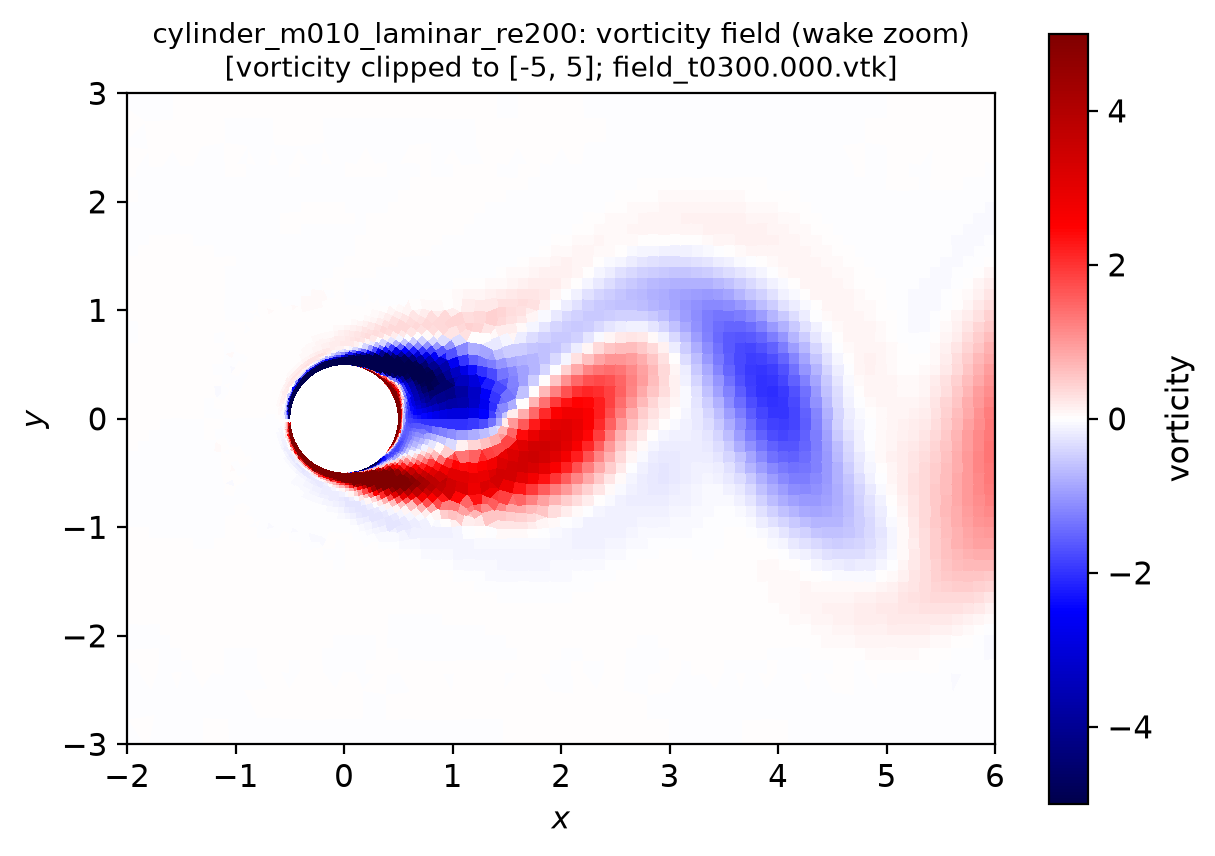
\includegraphics[width=0.7\linewidth]{figures/cylinder_m010_laminar_re200_vorticity_wake.png}
\caption{Cylinder laminar, $M_\infty=0.1$, $Re=200$ (vortex shedding): post-transient vorticity wake (clipped to $[-5,5]$).}\label{fig:cylinder_m010_laminar_re200_vorticity_wake}\end{figure}

The cylinder at $Re=200$ is run as a true BDF2 dual-time transient ($\Delta t=0.01$, $t_f=300$, $30{,}000$ physical steps, inner LU-SGS solve to a $10^{-3}$ total-residual reduction per step). After the initial transient a self-sustained von K\'arm\'an vortex street develops: the lift oscillates periodically (Fig.~\ref{fig:cylinder_m010_laminar_re200_forces}) and the post-transient vorticity field (Fig.~\ref{fig:cylinder_m010_laminar_re200_vorticity_wake}) shows the alternating signed vortices convecting downstream. The measured Strouhal number, mean drag, and lift amplitude are reported in the summary line above and in Table~\ref{tab:results}; the shedding frequency is extracted from the post-transient lift history by an FFT. The drag magnitude is under-predicted relative to incompressible references ($C_D\approx1.3$) owing to low-Mach dissipation (\S\ref{sec:limitations}), but the shedding frequency and flow structure are correct.